\RequirePackage[l2tabu,orthodox]{nag}

% two-sided
\documentclass[headsepline,footsepline,footinclude=false,fontsize=11pt,paper=a4,listof=totoc,bibliography=totoc,BCOR=12mm,DIV=12]{scrbook} % two-sided
% \documentclass[headsepline,footsepline,footinclude=false,oneside,fontsize=11pt,paper=a4,listof=totoc,bibliography=totoc]{scrbook} % one-sided

\PassOptionsToPackage{table,svgnames,dvipsnames}{xcolor}

\usepackage[utf8]{inputenc}
\usepackage[T1]{fontenc}
\usepackage[sc]{mathpazo}
\usepackage[ngerman,american]{babel}
\usepackage[autostyle]{csquotes}
\usepackage[%
  backend=biber,
  url=false,
  sorting=ynt,
  style=numeric,
  maxnames=4,
  minnames=3,
  maxbibnames=99,
  giveninits,
  uniquename=init]{biblatex}
\usepackage{graphicx}
\usepackage{scrhack} % necessary for listings package
\usepackage{listings}
\usepackage{lstautogobble}
\usepackage{tikz}
\usepackage{pgfplots}
\usepackage{pgfplotstable}
\usepackage{booktabs}
\usepackage[final]{microtype}
\usepackage{caption}
\usepackage[hidelinks]{hyperref} % hidelinks removes colored boxes around references and links
\usepackage{amsmath}
\usepackage{mathtools}
\usepackage{amsthm,thmtools}
\usepackage[nottoc]{tocbibind}
\usepackage[ruled]{algorithm2e}
\usepackage{enumerate}
\usepackage{tabularx}
% \usepackage{ltablex}
\usepackage{imakeidx}

\DeclareMathOperator*{\argmax}{arg\,max}
\DeclareMathOperator*{\argmin}{arg\,min}

\makeindex[intoc]

\DeclarePairedDelimiter{\norm}{\lVert}{\rVert}

\declaretheorem[name=Theorem]{theorem}
\declaretheorem[name=Lemma,sibling=theorem]{lemma}
\declaretheorem[name=Definition,sibling=theorem]{definition}
\declaretheorem[name=Problem,sibling=theorem]{problem}
\makeatletter
\def\ll@problem{
  \protect\numberline{\theproblem}\thmt@shortoptarg
}
\makeatother

\renewcommand{\thealgocf}{\arabic{theorem}}

\bibliography{sources}

\setkomafont{disposition}{\normalfont\bfseries} % use serif font for headings
\linespread{1.05} % adjust line spread for mathpazo font

% Add table of contents to PDF bookmarks
\BeforeTOCHead[toc]{{\cleardoublepage\pdfbookmark[0]{\contentsname}{toc}}}

% Define TUM corporate design colors
% Taken from http://portal.mytum.de/corporatedesign/index_print/vorlagen/index_farben
\definecolor{TUMBlue}{HTML}{0065BD}
\definecolor{TUMSecondaryBlue}{HTML}{005293}
\definecolor{TUMSecondaryBlue2}{HTML}{003359}
\definecolor{TUMBlack}{HTML}{000000}
\definecolor{TUMWhite}{HTML}{FFFFFF}
\definecolor{TUMDarkGray}{HTML}{333333}
\definecolor{TUMGray}{HTML}{808080}
\definecolor{TUMLightGray}{HTML}{CCCCC6}
\definecolor{TUMAccentGray}{HTML}{DAD7CB}
\definecolor{TUMAccentOrange}{HTML}{E37222}
\definecolor{TUMAccentGreen}{HTML}{A2AD00}
\definecolor{TUMAccentLightBlue}{HTML}{98C6EA}
\definecolor{TUMAccentBlue}{HTML}{64A0C8}

% Settings for pgfplots
\pgfplotsset{compat=newest}
\pgfplotsset{
  % For available color names, see http://www.latextemplates.com/svgnames-colors
  cycle list={TUMBlue\\TUMAccentOrange\\TUMAccentGreen\\TUMSecondaryBlue2\\TUMDarkGray\\},
}

% Settings for lstlistings
\lstset{%
  basicstyle=\ttfamily,
  columns=fullflexible,
  autogobble,
  keywordstyle=\bfseries\color{TUMBlue},
  stringstyle=\color{TUMAccentGreen}
}

% Colors
\def\b{\textcolor{blue}}
\def\r{\textcolor{red}}

% Ternary operator
\newcommand{\ternary}[3]{\textbf{if}\ #1\ \textbf{then}\ #2\ \textbf{else}\ #3}


% thesis information
\newcommand*{\getUniversity}{Technical University of Munich}
\newcommand*{\getFaculty}{Department of Informatics}
\newcommand*{\getTitle}{Implementation of Algorithms for Right-Sizing Data Centers}
\newcommand*{\getTitleGer}{Implementierung von Algorithmen für die Größenanpassung von Rechenzentren}
\newcommand*{\getAuthor}{Jonas Hübotter}
\newcommand*{\getDoctype}{Bachelor's Thesis in Informatics}
\newcommand*{\getSupervisor}{Prof. Dr. Susanne Albers}
\newcommand*{\getAdvisor}{Jens Quedenfeld}
\newcommand*{\getSubmissionDate}{July 31, 2021}
\newcommand*{\getSubmissionLocation}{Munich}

\makenoidxglossaries

% basic notation
\glsxtrnewsymbol[description={\ensuremath{\{1, \dots, n\}}, for \ensuremath{n \in \mathbb{N}}}]{range}{\ensuremath{[n]}}
\glsadd{range}
\glsxtrnewsymbol[description={\ensuremath{\{0\} \cup [n]}, for \ensuremath{n \in \mathbb{N}}}]{0range}{\ensuremath{[n]_0}}
\glsadd{0range}
\glsxtrnewsymbol[description={\ensuremath{\max\{0, x\}}, for \ensuremath{x \in \mathbb{R}}}]{positive}{\ensuremath{(x)^+}}
\glsadd{positive}
\glsxtrnewsymbol[description={smallest entry of the vector \ensuremath{x}}]{vec_min}{\ensuremath{x_{min}}}
\glsadd{vec_min}
\glsxtrnewsymbol[description={largest entry of the vector \ensuremath{x}}]{vec_max}{\ensuremath{x_{max}}}
\glsadd{vec_max}

% symbols


\begin{document}

% Set page numbering to avoid "destination with the same identifier has been already used" warning for cover page.
% (see https://en.wikibooks.org/wiki/LaTeX/Hyperlinks#Problems_with_Links_and_Pages).
\pagenumbering{alph}
\begin{titlepage}
  % HACK for two-sided documents: ignore binding correction for cover page.
  % Adapted from Markus Kohm's KOMA-Script titlepage=firstiscover handling.
  % See http://mirrors.ctan.org/macros/latex/contrib/koma-script/scrkernel-title.dtx,
  % \maketitle macro.
  \oddsidemargin=\evensidemargin\relax
  \textwidth=\dimexpr\paperwidth-2\evensidemargin-2in\relax
  \hsize=\textwidth\relax

  \centering
  \null
  \vspace{18mm}
  \IfFileExists{thesis/logos/tum.pdf}{%
    
\includegraphics[height=20mm]{thesis/logos/tum.pdf}
  }{%
    \vspace*{20mm}
  }

  \vspace{10mm}
  {\huge\MakeUppercase{\getFaculty{}}}\\

  \vspace{5mm}
  {\large\MakeUppercase{\getUniversity{}}}\\

  \vspace{20mm}
  {\Large \getDoctype{}}

  \vspace{15mm}
  {\huge\bfseries \getTitle{}}

  \vspace{15mm}
  {\LARGE \getAuthor{}}

  \IfFileExists{thesis/logos/faculty.pdf}{%
    \vfill{}
    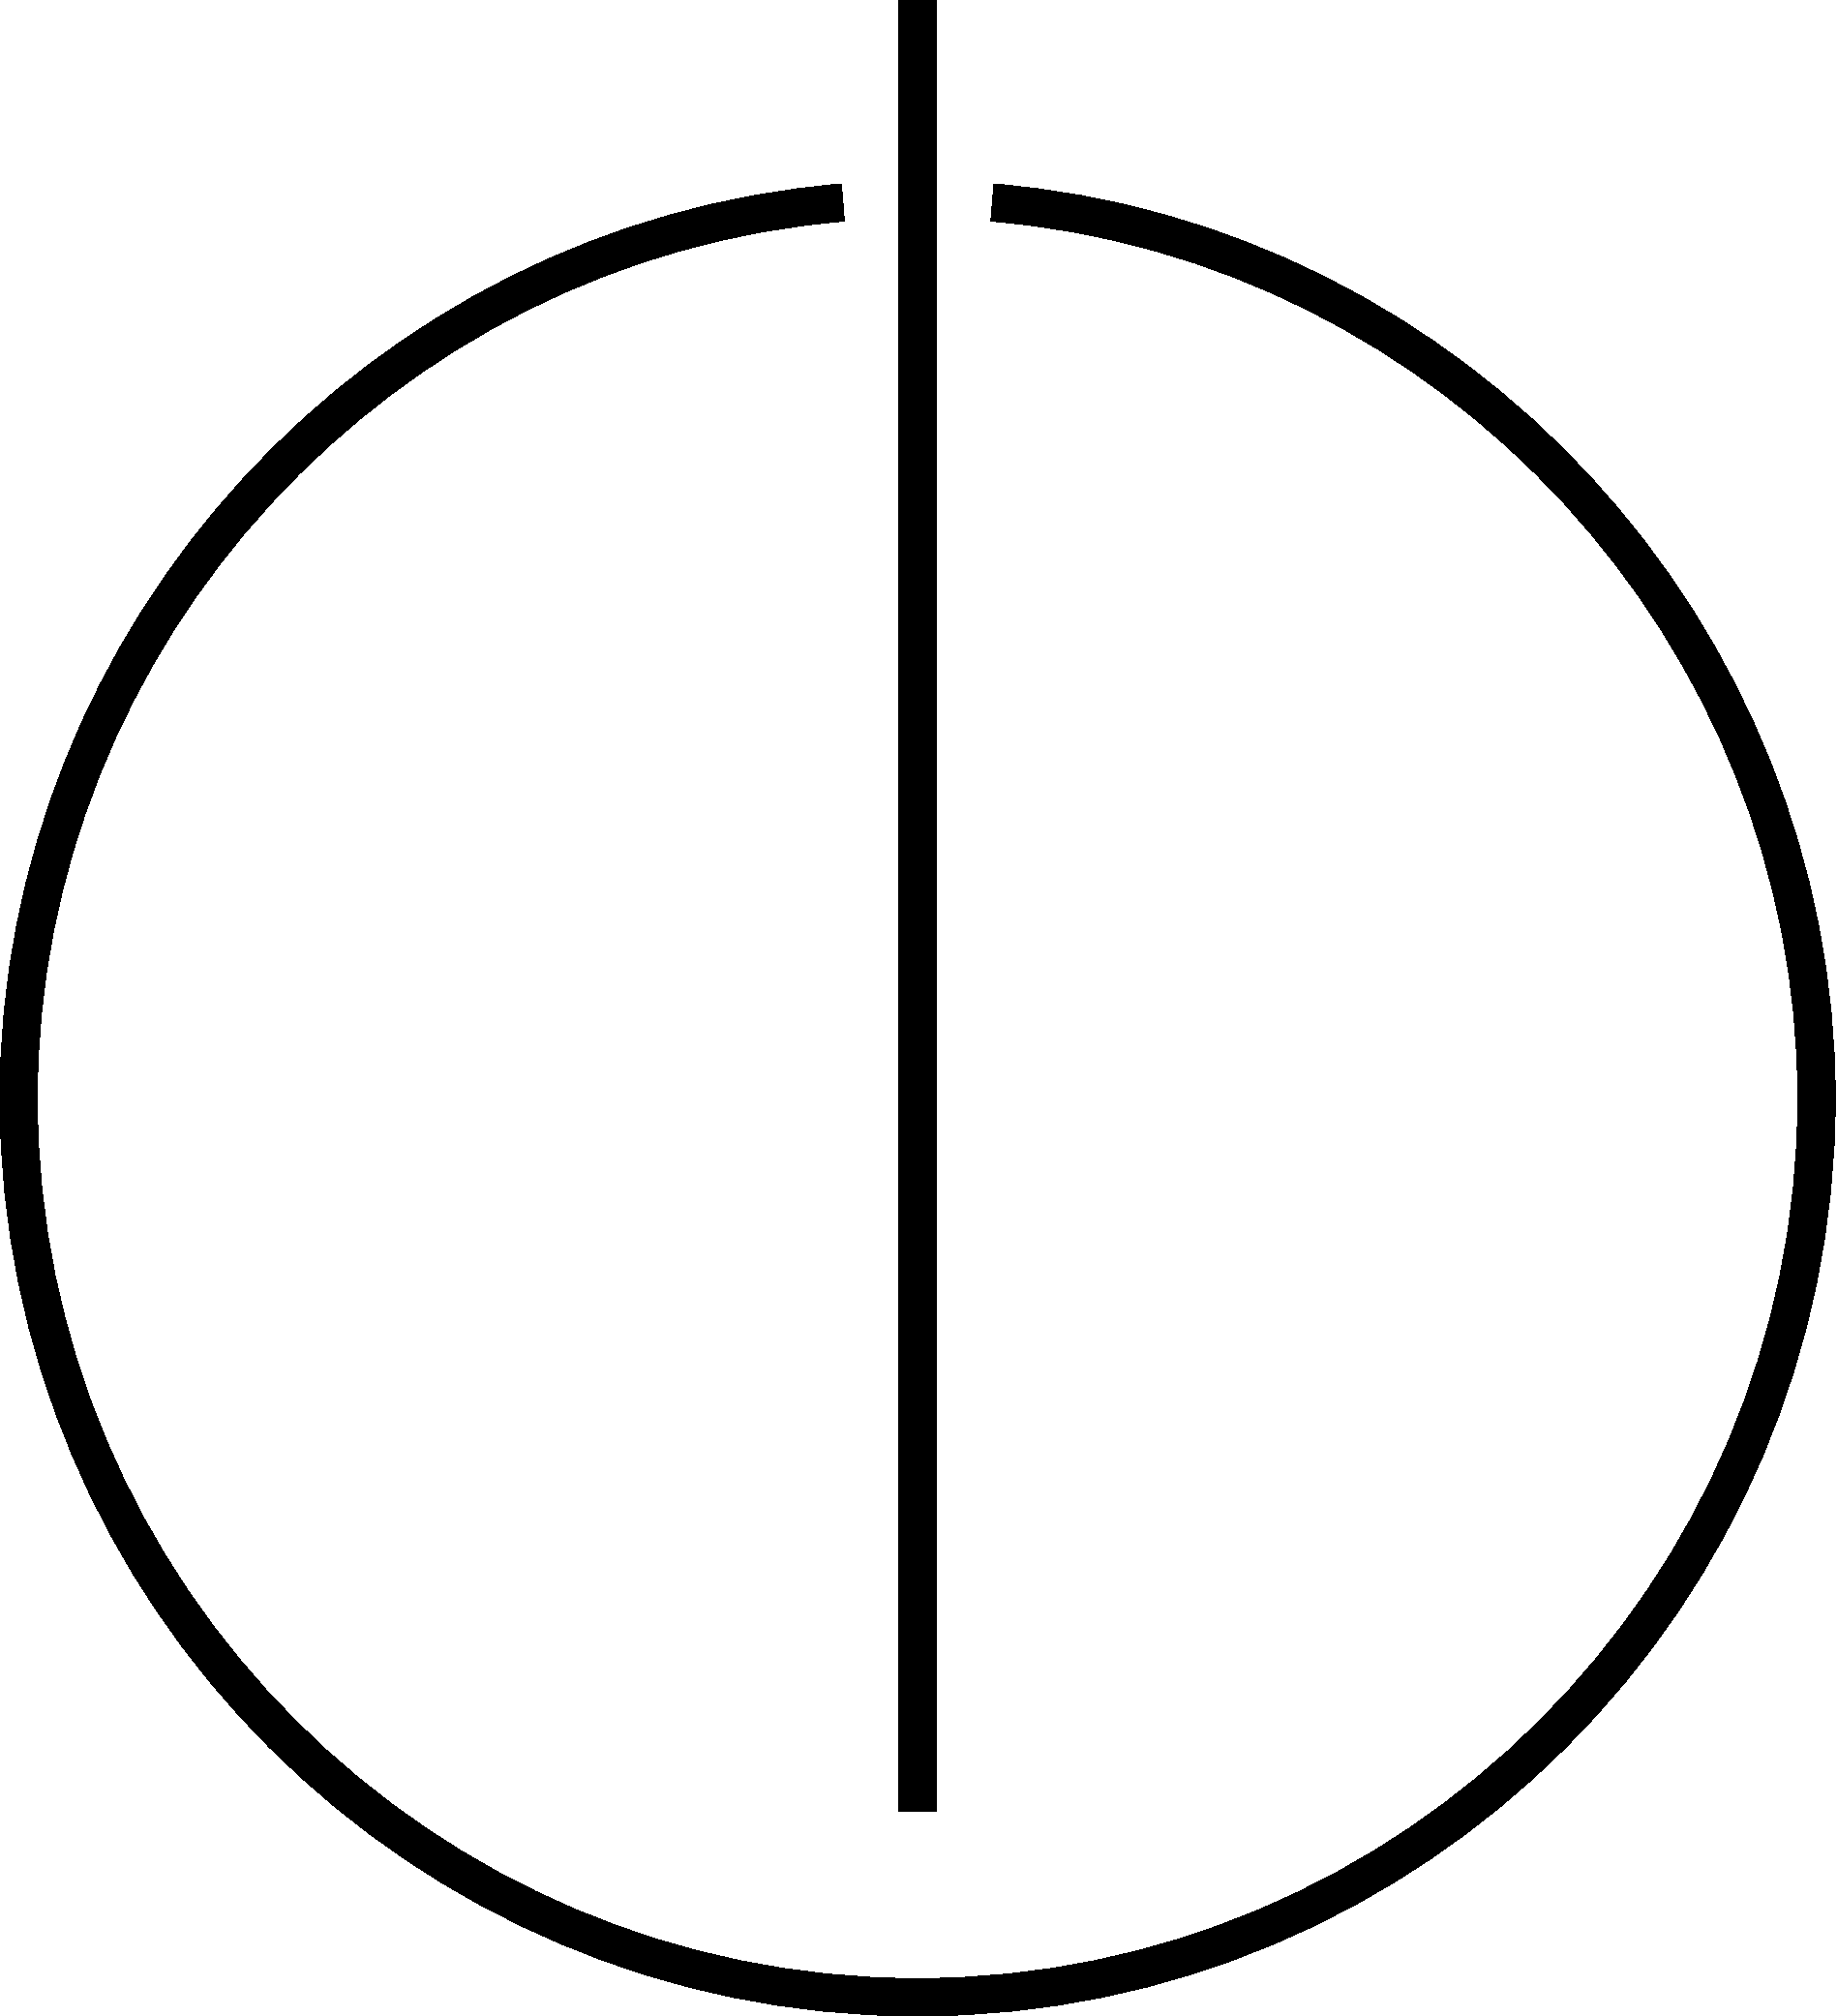
\includegraphics[height=20mm]{thesis/logos/faculty.pdf}
  }{}
\end{titlepage}

\frontmatter{}

\begin{titlepage}
  \centering

  \IfFileExists{thesis/logos/tum.pdf}{%
    
\includegraphics[height=20mm]{thesis/logos/tum.pdf}
  }{%
    \vspace*{20mm}
  }

  \vspace{10mm}
  {\huge\MakeUppercase{\getFaculty{}}}\\

  \vspace{5mm}
  {\large\MakeUppercase{\getUniversity{}}}\\

  \vspace{20mm}
  {\Large \getDoctype{}}

  \vspace{15mm}
  {\huge\bfseries \getTitle{}}

  \vspace{10mm}
  {\huge\bfseries \foreignlanguage{ngerman}{\getTitleGer{}}}

  \vspace{15mm}
  \begin{tabular}{l l}
    Author:          & \getAuthor{} \\
    Supervisor:      & \getSupervisor{} \\
    Advisor:         & \getAdvisor{} \\
    Submission Date: & \getSubmissionDate{} \\
  \end{tabular}

  \vspace{6mm}
  \IfFileExists{thesis/logos/faculty.pdf}{%
    \vfill{}
    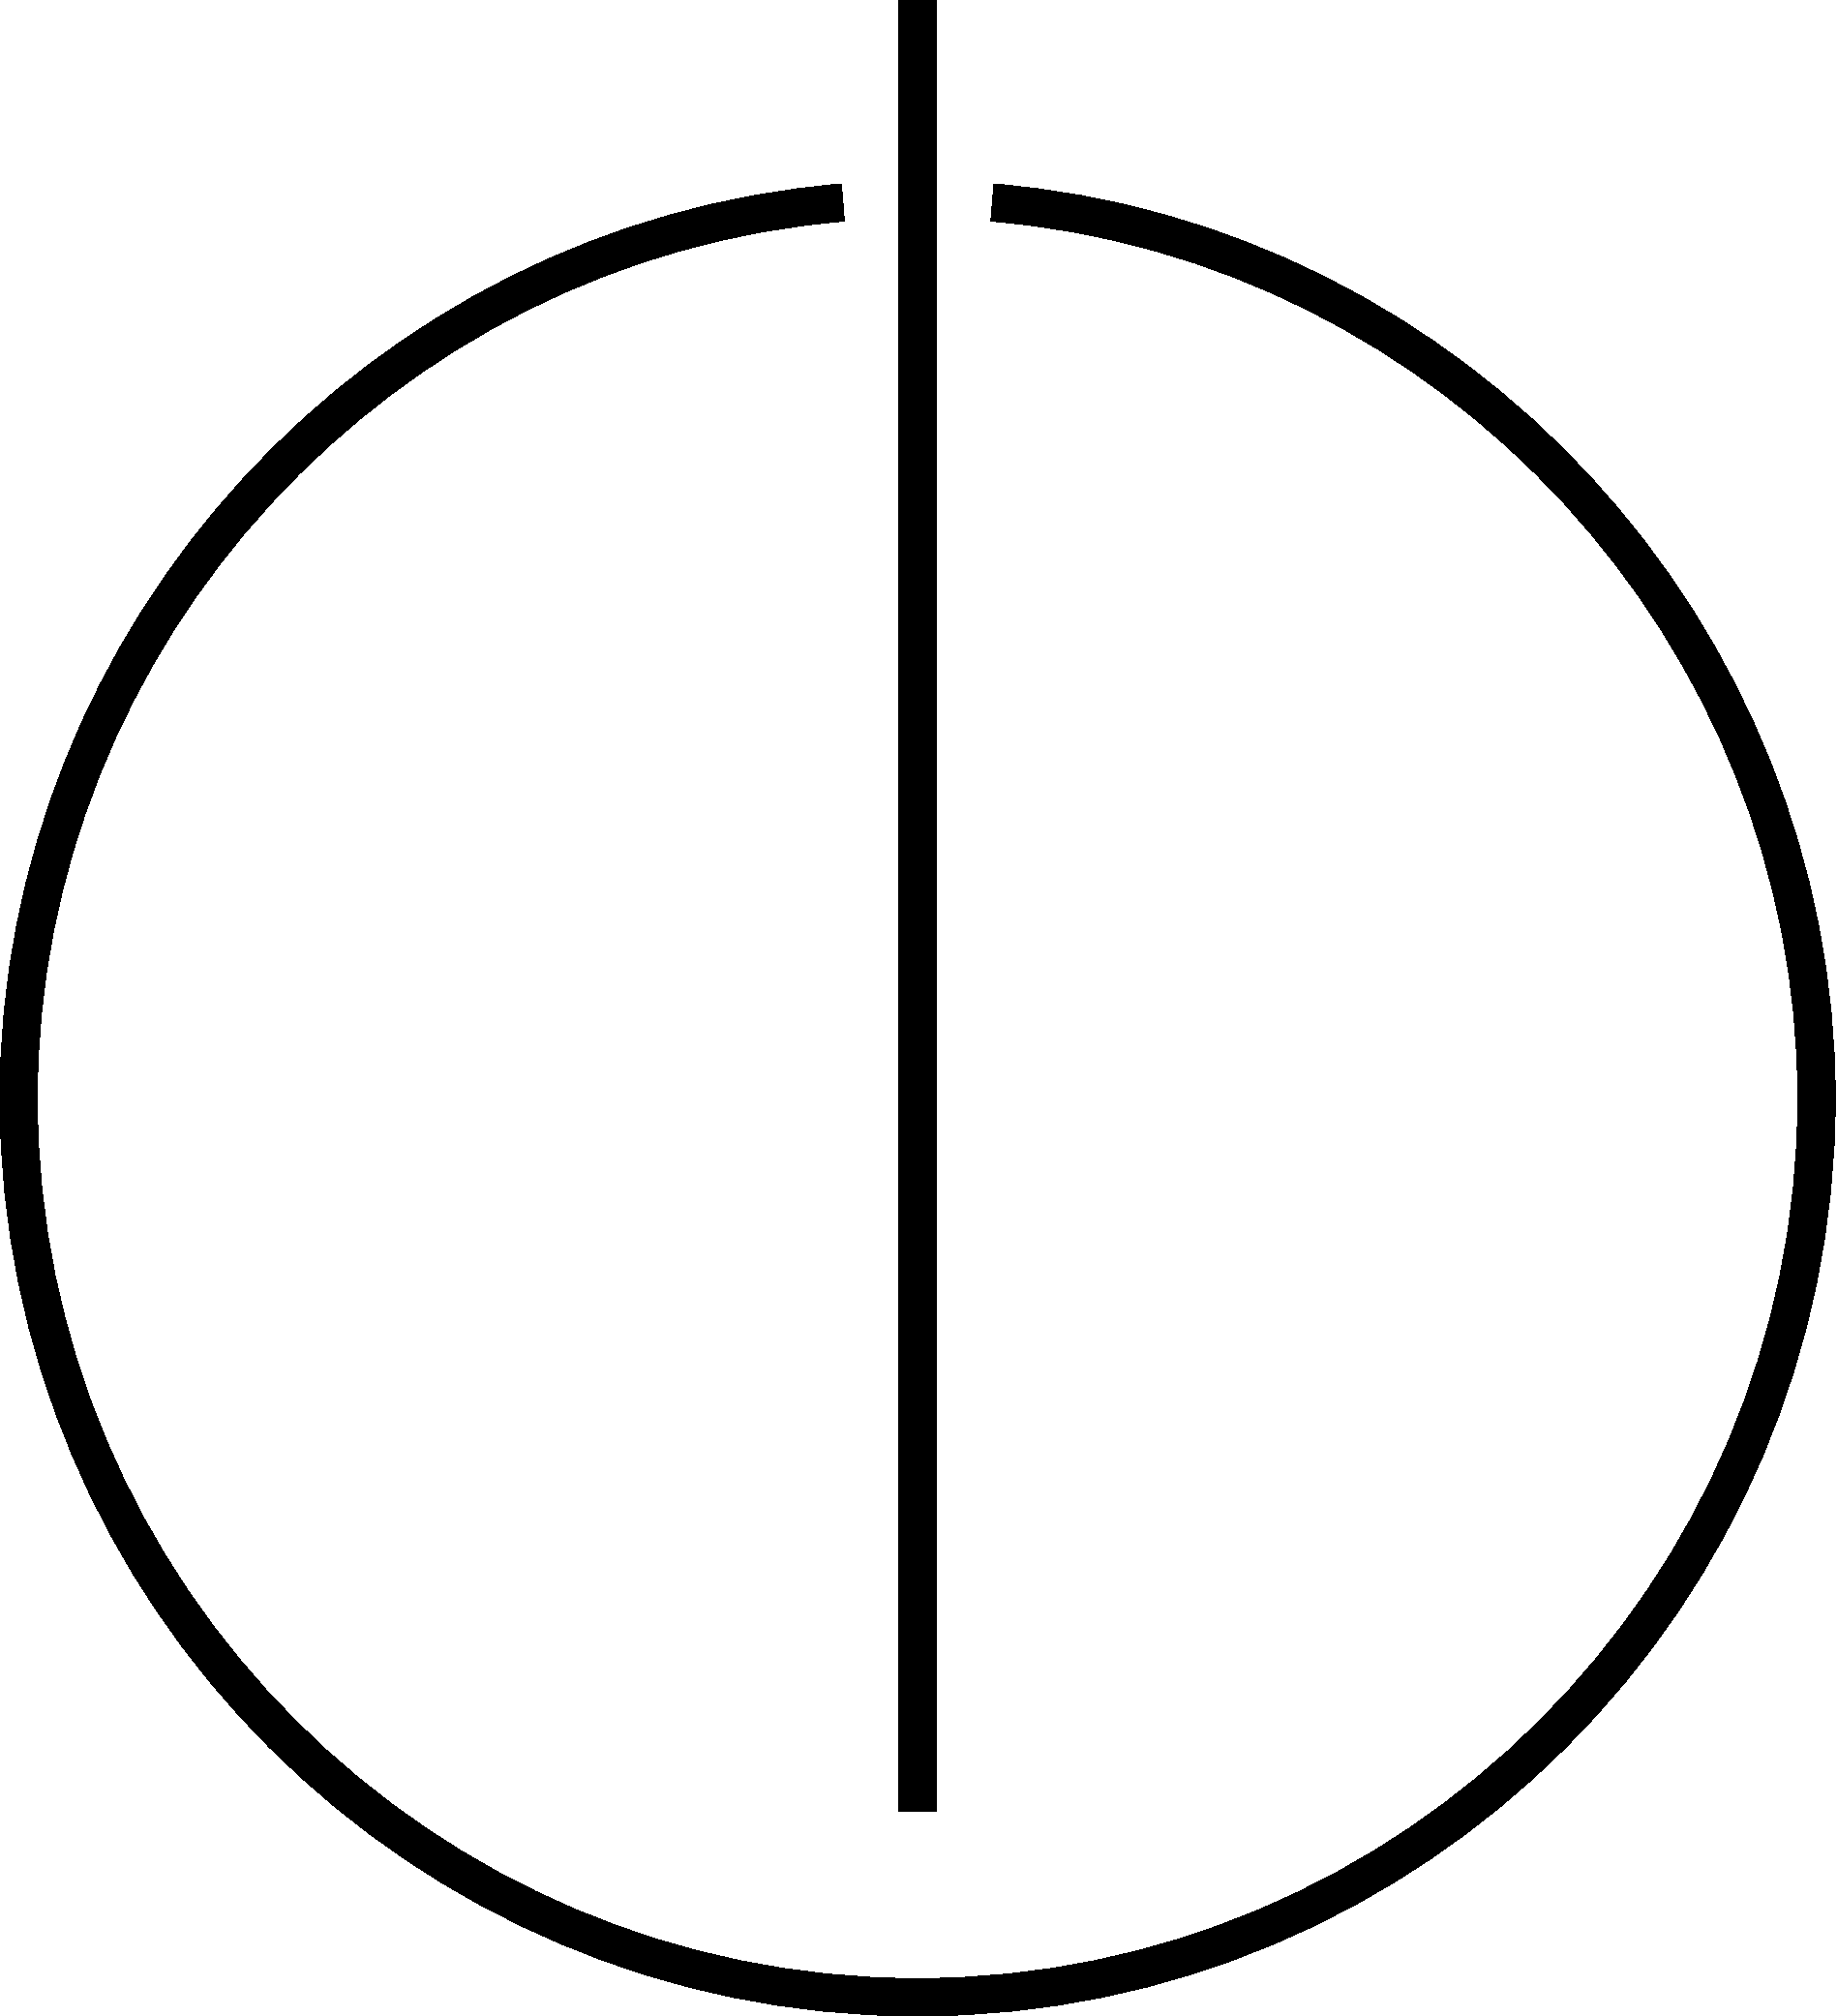
\includegraphics[height=20mm]{thesis/logos/faculty.pdf}
  }{}
\end{titlepage}
\cleardoublepage{}

\thispagestyle{empty}
\vspace*{0.8\textheight}
\noindent
I confirm that this bachelor's thesis is my own work and I have documented all sources and material used.

\vspace{15mm}
\noindent
\getSubmissionLocation{}, \getSubmissionDate{} \hspace{50mm} \getAuthor{}

\cleardoublepage{}

\addcontentsline{toc}{chapter}{Acknowledgments}
\thispagestyle{empty}

\vspace*{20mm}

\begin{center}
{\usekomafont{section} Acknowledgments}
\end{center}

\vspace{10mm}

%TODO: Acknowledgments

\cleardoublepage{}

\chapter{\abstractname}

The energy consumption of data centers assumes a significant fraction of the worlds overall energy consumption. Most data centers are statically provisioned leading to a very low average utilization of servers. In this work we survey uni-dimensional and high-dimensional approaches for dynamically powering-up and powering-down servers to reduce the energy footprint of data centers while ensuring that incoming jobs are processed in-time. We implement algorithms for smoothed online convex optimization and variations thereof where in each round the agent receives a convex cost function. The agent seeks to minimize cost based on an exploration-exploitation trade-off using an additional switching cost which is associated with changing decisions in-between rounds. We implement the algorithms in their most general form, inviting future research on their performance in other application areas. We evaluate the algorithms for the application of right-sizing data centers using traces from Facebook, Microsoft, Alibaba, and Los Alamos National Lab. Our experiments show that the the online algorithms perform close to the dynamic offline optimum in practice and promise a significant cost reduction when compared to the static offline optimum. We discuss how features of the data center model and trace impact the performance. Finally, we investigate the practical use of predictions to achieve further cost reductions.

\microtypesetup{protrusion=false}
\tableofcontents{}
\microtypesetup{protrusion=true}

\mainmatter{}

% !TeX root = ../main.tex
% Add the above to each chapter to make compiling the PDF easier in some editors.

\chapter{Introduction}\label{chapter:introduction}

\section{Section}
Citation test~\parencite{latex}.

\subsection{Subsection}

See~\autoref{tab:sample}, \autoref{fig:sample-drawing}, \autoref{fig:sample-plot}, \autoref{fig:sample-listing}.

\begin{table}[htpb]
  \caption[Example table]{An example for a simple table.}\label{tab:sample}
  \centering
  \begin{tabular}{l l l l}
    \toprule
      A & B & C & D \\
    \midrule
      1 & 2 & 1 & 2 \\
      2 & 3 & 2 & 3 \\
    \bottomrule
  \end{tabular}
\end{table}

\begin{figure}[htpb]
  \centering
  % This should probably go into a file in figures/
  \begin{tikzpicture}[node distance=3cm]
    \node (R0) {$R_1$};
    \node (R1) [right of=R0] {$R_2$};
    \node (R2) [below of=R1] {$R_4$};
    \node (R3) [below of=R0] {$R_3$};
    \node (R4) [right of=R1] {$R_5$};

    \path[every node]
      (R0) edge (R1)
      (R0) edge (R3)
      (R3) edge (R2)
      (R2) edge (R1)
      (R1) edge (R4);
  \end{tikzpicture}
  \caption[Example drawing]{An example for a simple drawing.}\label{fig:sample-drawing}
\end{figure}

\begin{figure}[htpb]
  \centering

  \pgfplotstableset{col sep=&, row sep=\\}
  % This should probably go into a file in data/
  \pgfplotstableread{
    a & b    \\
    1 & 1000 \\
    2 & 1500 \\
    3 & 1600 \\
  }\exampleA
  \pgfplotstableread{
    a & b    \\
    1 & 1200 \\
    2 & 800 \\
    3 & 1400 \\
  }\exampleB
  % This should probably go into a file in figures/
  \begin{tikzpicture}
    \begin{axis}[
        ymin=0,
        legend style={legend pos=south east},
        grid,
        thick,
        ylabel=Y,
        xlabel=X
      ]
      \addplot table[x=a, y=b]{\exampleA};
      \addlegendentry{Example A};
      \addplot table[x=a, y=b]{\exampleB};
      \addlegendentry{Example B};
    \end{axis}
  \end{tikzpicture}
  \caption[Example plot]{An example for a simple plot.}\label{fig:sample-plot}
\end{figure}

\begin{figure}[htpb]
  \centering
  \begin{tabular}{c}
  \begin{lstlisting}[language=SQL]
    SELECT * FROM tbl WHERE tbl.str = "str"
  \end{lstlisting}
  \end{tabular}
  \caption[Example listing]{An example for a source code listing.}\label{fig:sample-listing}
\end{figure}

% !TeX root = ../main.tex
% Add the above to each chapter to make compiling the PDF easier in some editors.

\chapter{Theory}\label{chapter:theory}

\section{Problems}

\subsection{Smoothed Convex Optimization}

\begin{problem}[Smoothed Convex Optimization (SCO)]
Given a time horizon $T \in \mathbb{N}$, a convex decision space $\mathcal{X} \subset \mathbb{R}^d$, a norm $\norm{\cdot}$ on $\mathbb{R}^d$, and a sequence of non-negative convex functions $f_t$ for $t \in [T]$ with $f_t(x) = \infty$ for all $x \not\in \mathcal{X}$, find $x \in \mathcal{X}$ minimizing \begin{align*}
    c(x) = \sum_{t=1}^T f_t(x_t) + \norm{x_t - x_{t-1}}
\end{align*}
where $x_0 = 0$.
\end{problem}

In many practical applications of Smoothed Convex Optimization, we seek to find integral solutions minimizing hitting and switching costs. This is especially true within the context of resource allocation, for example for right-sizing data centers, where our resources are discrete. This observation motivates the definition of the following variant of SCO.

\begin{problem}[Integral Smoothed Convex Optimization (Int-SCO)]
We define Integral Smoothed Convex Optimization analogously to SCO with the added restriction that the points $x$ in $d$-dimensional space must be discrete, that is $\mathcal{X} \subset \mathbb{Z}^d$.
\end{problem}

\subsubsection{Complexity of the Offline Problem}

We now want to examine the complexity of Int-SCO in the offline case. That is, we know all arriving convex cost functions $f_t$ in advance. We prove Int-SCO NP-hard for varying $d$ by giving a polynomial-time reduction from the Knapsack problem. In \autoref{section:theory:simplified_smoothed_convex_optimization} we first extend this proof of NP-hardness to the Integral Simplified Smoothed Convex Optimization problem which restricts the decision space and switching cost. Then, in \autoref{section:theory:smoothed_balanced_load_optimization}, we extend the proof to the Integral Smoothed Balanced-Load Optimization problem which further restricts the structure of the cost functions.

Given a set of items with an associated value and weight and an upper bound to the total weight, Knapsack is the problem of determining the number of copies of each item that maximizes the total value and conforms to the given upper bound on total weight. Formally we define Knapsack as follows.

\begin{problem}[Knapsack (KP)]
Given a number of items $n \in \mathbb{N}$, a value of each item $v \in \mathbb{N}^n$, a weight of each item $w \in \mathbb{N}^n$, and an upper bound to the total weight $W \in \mathbb{N}$, find $x \in \{0,1\}^n$ satisfying $\sum_{i = 1}^n w_i x_i \leq W$ and maximizing $\sum_{i=1}^n v_i x_i$.
is maximized.
\end{problem}

This variant of Knapsack is commonly called \textit{0-1 Knapsack} and restricts the number of copies of each item to be either 0 or 1. It is, however, easy to see that our proof can easily be generalized to a setting where we allow $x_i \in [m_i]_0$ for $m \in \mathbb{N}^n$. TODO et al. show that the Knapsack decision problem is NP-complete and that the Knapsack optimization problem is NP-hard.

Before reducing to Int-SCO, we reduce Knapsack to a related problem called Minimum Knapsack.

\begin{problem}[Minimum Knapsack (Min-KP)]
Given a number of items $n \in \mathbb{N}$, a cost of each item $c \in \mathbb{N}^n$, a utility of each item $u \in \mathbb{N}^n$, and a lower bound to the total utility $U \in \mathbb{N}$, find $x \in \{0,1\}^n$ satisfying $\sum_{i = 1}^n u_i x_i \geq U$ and minimizing $\sum_{i=1}^n c_i x_i$.
\end{problem}

\begin{lemma}
Min-KP is NP-hard.
\end{lemma}

\begin{proof}
We prove the lemma by giving a reduction from KP.

Let $\mathcal{I}_1 = (n, v, w, W)$ be an instance of KP. Let $\mathcal{I}_2(U) = (n, c, u, U)$ be an instance of Min-KP with $c = w$, and $u = v$. Hence, $\mathcal{I}_2(U)$ minimizes the total weight $\sum_{i=1}^n w_i x_i$ such that $\sum_{i=1}^n v_i x_i \geq U$.

By finding solutions to $\mathcal{I}_2(U)$ repeatedly for varying $U$, we determine the maximal $U$ such that $\sum_{i=1}^n w_i x_i \leq W$. Let $v_{max} = \max\{v_i \mid i \in [n]\}$ be the maximal value of any item. We observe that $U$ is upper bounded by $n \cdot v_{max}$. If $U$ were greater than $n \cdot v_{max}$ we would have $\sum_{i=1}^n v_{max} x_i \geq \sum_{i=1}^n v_i x_i > n \cdot v_{max}$ which contradicts $x \in \{0,1\}^n$. Hence, we can use binary search to find $U$ in $\mathcal{O}(\log n + \log v_{max})$ iterations. The other direction works analogously.

We have seen a total, polynomial-time reduction from KP to Min-KP. Hence, Min-KP is NP-hard.
\end{proof}

Next we prove our main reduction from Min-KP to Int-SCO. To motivate this reduction, we first prove that the following (convex) integer optimization is in fact equivalent to Min-KP.

\begin{lemma}
\label{lemma:integer_minimization}
Let $\mathcal{I} = (n, c, u, U)$ be an instance of Min-KP. $x$ is the solution to $\mathcal{I}$ if and only if $x$ minimizes \begin{align*}
    c'(x) = \sum_{i=1}^n c_i x_i + M(U - \sum_{i=1}^n u_i x_i)^+
\end{align*} subject to $x \in \{0,1\}^n$ for some $M > \frac{c_{max}}{u_{min}}$.
\end{lemma}

\begin{proof}
Suppose $x$ minimizes $c'(x)$. Now suppose $(U - \sum_{i=1}^n u_i x_i)^+ > 0$. Then, $(U - \sum_{i=1}^n u_i x_i)^+ \geq u_{min}$. Therefore, $c'(x) > \sum_{i=1}^n c_i x_i + c_{max}$. We observe that $x$ is not optimal as either $c'(x)$ could be minimized further by increasing $x$ such that $(U - \sum_{i=1}^n u_i x_i)^+ = 0$ since $\sum_{i=1}^n c_i x_i \leq c_{max}$ holds for all $x$. Alternatively, $x$ already equals 1 in each dimension in which case $\sum_{i=1}^n u_i < U$, indicating that $\mathcal{I}$ has no solution.

By leading our previous assumption to a contradiction, we conclude $(U - \sum_{i=1}^n u_i x_i)^+ = 0$ and therefore $U \leq \sum_{i=1}^n u_i x_i$. Further, $c'(x)$ minimizes $\sum_{i=1}^n c_i x_i$ for all remaining candidates for $x$. Hence, $x$ is the solution of $\mathcal{I}$.

On the other hand, suppose that $x$ is the solution to $\mathcal{I}$. Then $(U - \sum_{i=1}^n u_i x_i)^+ = 0$ and $\sum_{i=1}^n c_i x_i$ is minimized. Hence, $x$ minimizes $c'(x)$.
\end{proof}

For our construction we need that $c$ is convex.

\begin{lemma}
\label{lemma:integer_minimization_convexity}
$c'(\cdot)$ is convex.
\end{lemma}

\begin{proof}
It is easy to see that $c$ is continuous. Therefore, to show the convexity of $c$ it suffices to prove $c'(\frac{x+y}{2}) \leq \frac{c'(x)+c'(y)}{2}$ for all $x, y \in \mathbb{R}^n$.

To simplify the notation let $c'(x) = \sum_{i=1}^n c_i x_i$ and let $U(x) = \sum_{i=1}^n u_i x_i$. To further simplify the notation we define $\frac{x+y}{2}$ to be applied component-wise to elements $i \in [n]$ of $x$ and $y$. We then obtain \small{
\begin{align*}
         &c'(\frac{x+y}{2}) \leq \frac{c'(x)+c'(y)}{2} \\
    \iff &C(\frac{x+y}{2}) + M(U - U(\frac{x+y}{2}))^+ \leq \frac{C(x) + M(U - U(x))^+ + C(y) + M(U - U(y))^+}{2} \\
    \iff &C(x) + C(y) + 2M(U - U(\frac{x+y}{2}))^+ \leq C(x) + M(U - U(x))^+ + C(y) + M(U - U(y))^+ \\
    \iff &2(U - U(\frac{x+y}{2}))^+ \leq (U - U(x))^+ + (U - U(y))^+.
\end{align*}
}\normalsize

We immediately get the convexity of $U(\cdot)$ by the following equivalence. \begin{align*}
    U(\frac{x+y}{2}) &= \sum_{i=1}^n u_i \frac{x_i + y_i}{2} \\
                     &= \frac{\sum_{i=1}^n u_i x_i + \sum_{i=1}^n u_i y_i}{2} \\
                     &= \frac{U(x) + U(y)}{2}.
\end{align*}

Now, we consider three cases separately.

\begin{enumerate}
    \item If $U(x) > U$ and $U(y) > U$, then $U(\frac{x+y}{2}) > U$. Hence \begin{align*}
        2(U - U(\frac{x+y}{2}))^+ = 0 = (U - U(x))^+ + (U - U(y))^+.
    \end{align*}
    \item If $U(x) \leq U$ and $U(y) \leq U$, then $U(\frac{x+y}{2}) \leq U$. Hence \begin{align*}
        2(U - U(\frac{x+y}{2}))^+ &= 2U - 2U(\frac{x+y}{2}) \\
                                  &= 2U - U(x) + U(y) \\
                                  &= (U - U(x))^+ + (U - U(y))^+.
    \end{align*}
    \item For the only remaining case we assume w.l.o.g. that $U(x) \leq U$ and $U(y) > U$. If $U - U(x) < U(y) - U$, then $U(\frac{x+y}{2}) > U$ and we follow the first case. If, on the other hand, $U - U(x) \geq U(y) - U$, then $U(\frac{x+y}{2}) \leq U$ and we follow the second case.\qedhere
\end{enumerate}
\end{proof}

We now have everything in place to prove our main result of this section.

\begin{theorem}
Int-SCO is NP-hard.
\end{theorem}

\begin{proof}
We now give our reduction from Min-KP to Int-SCO.

Let $\mathcal{I}_1 = (n, c, u, U)$ be an instance of Min-KP. We define $\mathcal{I}_2 = (T, \mathcal{X}, \norm{\cdot}, f)$ as an instance of Int-SCO with $T = 1$, $\mathcal{X} = \{0,1\}^n$, $\norm{\cdot} = 0$, and $f_1(x) = c'(x)$. We further set $d = n$. By \autoref{lemma:integer_minimization_convexity}, $\mathcal{I}_2$ is a valid instance of Int-SCO.

The correctness of our construction follows from \autoref{lemma:integer_minimization}.

\begin{align*}
         &x \text{ is a solution to } \mathcal{I}_2 \\
    \iff &x \text{ minimizes } \sum_{t=1}^T f_t(x_t) + \norm{x_t - x_{t-1}} \text{ such that } x_t \in \mathcal{X}. \\
    \iff &x \text{ minimizes } c'(x_1) \text{ such that } x_1 \in \{0,1\}^n. \\
    \iff &x_1 \text{ is a solution to } \mathcal{I}_1.
\end{align*}

Our construction is total and polynomial in the size of $\mathcal{I}_1$. Hence, Int-SCO is NP-hard.
\end{proof}

We observe that the above reduction can be extended to Knapsack with arbitrary bounds $m_i$ by setting $\mathcal{X}$ of $\mathcal{I}_2$ to $[m_1]_0 \times \dots \times [m_n]_0$.

\subsection{Simplified Smoothed Convex Optimization}
\label{section:theory:simplified_smoothed_convex_optimization}

In many applications, for example for right-sizing data centers, it suffices to restrict $\mathcal{X}$ to $\mathcal{X} = [m_0]_0 \times \dots \times [m_d]_0$ for some $m \in \mathbb{N}^d$ and the switching cost $\norm{x}$ to $\sum_{k=1}^d \beta_k x_k^+$ where $\beta$ is constant for each dimension. To that end, we first define a restricted variant of (fractional) SCO which we term \textit{Simplified Smoothed Convex Optimization}.

\begin{problem}[Simplified Smoothed Convex Optimization (SSCO)]
Given a time horizon $T \in \mathbb{N}$, upper bounds $m \in \mathbb{N}^d$, switching costs $\beta \in \mathbb{R}_{>0}^d$, and a sequence of non-negative convex functions $f_t$ for $t \in [T]$, find $x \in \mathbb{R}_{\geq 0, \leq m_0} \times \dots \times \mathbb{R}_{\geq 0, \leq m_d}$ minimizing \begin{align*}
    c(x) = \sum_{t=1}^T f_t(x_t) + \sum_{k=1}^d \beta_k (x_{t,k} - x_{t-1,k})^+
\end{align*}
where $x_0 = 0$.
\end{problem}

We observe that $c(\cdot)$ pays the switching cost whenever $x$ increases. Decreasing $x$ does not increase the paid switching cost. This observation indicates that the following cost function $d(\cdot)$ is equivalent to $c(\cdot)$.

\begin{definition}[Inverted Simplified Smoothed Convex Optimization]
\begin{align*}
    d(x) = \sum_{t=1}^T f_t(x_t) + \sum_{k=1}^d \beta_k (x_{t,k} - x_{t+1,k})^+.
\end{align*}
Instead of $x_0 = 0$ we require $x_{T+1} = 0$.
\end{definition}

With the same motivation we used for the restriction of SCO to Int-SCO, we now restrict SSCO to an integral variant.

\begin{problem}[Integral Simplified Smoothed Convex Optimization (Int-SSCO)]
We define Integral Simplified Smoothed Convex Optimization analogously to SSCO with the added restriction that the points $x$ in $d$-dimensional space must be discrete, that is $x \in [m_0]_0 \times \dots \times [m_d]_0$.
\end{problem}

\subsubsection{Complexity of the Offline Problem}

We next extend our proof of NP-hardness of Int-SCO for varying $d$ to Int-SSCO. We cannot reuse our original proof as the switching cost of SSCO is required to be positive.

\subsection{Smoothed Balanced-Load Optimization}
\label{section:theory:smoothed_balanced_load_optimization}

\subsection{Smoothed Load Optimization}

\subsubsection{Complexity of the Offline Problem}

\section{Algorithm Analysis}

\subsection{Approximations}

\subsection{Regret}

\subsection{Competitiveness}

% !TeX root = ../main.tex
% Add the above to each chapter to make compiling the PDF easier in some editors.

\chapter{Application: Right-Sizing Data Centers}\label{chapter:application}

In this chapter we seek to derive models for right-sizing data centers based on smoothed convex optimization. We then use these models to motivate the variations of smoothed convex optimization we discussed in \autoref{chapter:theory}. We begin by discussing general features of server infrastructures. Then, we examine the modeling of \textit{operating costs} (i.e. hitting costs) and \textit{switching costs} in detail.

Data centers are large scale, complex systems. Therefore, any model we examine in this chapter is an approximation. Our goal is to find models that generalize well across many data centers. When examining a specific data center, the models we discuss can be extended to yield better approximations.

\section{Architectures}\label{section:application:architectures}

We begin by revisiting the characteristics by which the design of data centers varies.

\paragraph{Speed-Scalability} For our data center model it is natural to assume that the servers are speed scalable. That is, their utilization can vary from idling at 0\% utilization to full load at 100\% utilization. Furthermore, we assume that server utilization scales linearly with its load as that is required to maintain a constant quality of service \cite{Bansal2015}.

\paragraph{Energy} There has been much recent work on modeling the energy consumption of a data center as a function of speed of the individual servers. We discuss these approaches in detail in \autoref{section:application:operating_cost:energy}. However, in many cases the ecological and economical cost of energy does not remain constant. It fluctuates over time, but more importantly, at no single point in time is energy cost a linear function of energy consumption. This is because many data centers have quotas for each energy source \cite{Miller2021}. For example, there may only be a limited supply of renewable energy. Once the energy consumption of our data center exceeds this supply it has to resort to different sources of energy with different costs. Recently, a trend has also been for data centers to produce their own renewable energy \cite{Lin2012}. In this case, this renewable energy is significantly cheaper than any energy that may be purchased after consumption exceeds productions. If, in contrast, more energy is produced than is consumed, some energy may even be sold depending on the state of the energy grid.

\paragraph{Homogeneity and Heterogeneity} When the data center right-sizing problem was first introduced, approaches were focused on homogeneous data centers. In a \textit{homogeneous} data center, all servers are of the same type. We say that a server is of a different type than another server if their operating costs or switching costs differ significantly. In any such scenario where we have multiple server types, the data center is \textit{heterogeneous}. It is easy to see that each server type resembles one dimension in our smoothed optimization. While the model of a homogeneous data center is much simpler, in practice, most data centers are heterogeneous and this trend is projected to intensify \cite{Jin2016}. Heterogeneity may arise naturally as defect servers of a homogeneous data center are replaced by newer servers. The primary advantage of heterogeneous architectures is, however, that certain tasks can be delegated to specialized servers \cite{Jin2016}. For example, CPUs and GPUs may be used within the same data center but GPUs should only be used to perform massive parallel computations as CPUs are faster when tasks are more individual \cite{Shan2006}. The differing power-performance relationships of multiple server types are another benefit of heterogeneous architectures \cite{Jin2016}.

\paragraph{Size} In principle, the right-sizing data center problem only admits integral solutions, that is at any time we can only run an integral number of servers of each type. However, if the size of our data center is large in each dimension it is reasonable to use fractional solutions as an approximation. Typically, data centers fulfill this requirement. Lately, the surge in hyperscale facilities underlines that there is even a trend towards larger data centers \cite{Jones2018}. For this reason, discuss integral as well as fractional solutions in our analysis.

\paragraph{Reliability and Availability} Many services must satisfy certain requirements regarding reliability and availability, which are often key components of \textit{service level agreements} (SLAs) \cite{Lin2011}. In our model such requirements can be enforced as hard constraints using the decision space by requiring a minimum number of active servers per server type. As our model only chooses the number of servers of some type, the algorithm can then freely choose the active servers between all servers according to some guidelines to meet the requirements. However, choosing a decision space that is too tight, may reduce the cost saving potential. Therefore, an alternative approach is to use operating costs (discussed in \autoref{section:application:operating_cost}) as softer constraints, for example by enforcing a maximum utilization that is less than $\theta < 100\%$. Availability requirements for certain jobs can also be encoded into the revenue loss as a function of average job delay.

\paragraph{Networks} Most of our analysis is focused on the case of a single data center. However, the problem of deciding where to route incoming loads within a network of data centers so as to minimize the overall cost is an acutely relevant problem \cite{Miller2021}. For example, if data centers produce their own renewable energy, the cost of energy at each individual data center is likely to vary drastically over time as weather conditions shift \cite{Lin2012}. Therefore, previous studies focusing on individual data centers found that due to the intermittency of wind and solar they can only be used with large-scale storage \cite{Gmach2010, Gmach2010_2}. Yet, it has been shown that by running a network of data centers in separate locations the negative effects of renewable energy production can largely be avoided as the availability of solar and wind can be aggregated across locations \cite{Lin2012}. In \autoref{section:application:dynamic_routing}, we show how our cost model can be extended to support geographical load balancing across a network of data centers.

\section{Dispatching}\label{section:application:dispatching}

The modeling of load is the core of our data center model. We say that a \textit{load profile} of our system during time slot $t$ is a vector $\lambda_t \in \mathbb{N}_0^e$ where $e$ is the number of \textit{load types}. In the subsequent sections we give more concrete examples of varying load types, but generally loads are of different types when their cost model is different. For now, we assume that the processing time of all jobs on any server type takes exactly one time slot. In \autoref{section:application:dynamic_duration} we discuss in detail how this approach can be extended to jobs with a dynamic duration (per server type).

We denote by $m_k \in \mathbb{N}$ the maximum number of available servers of type $k$ and by $d$ the number of server types. Our decision space is therefore given as $\mathcal{X} := \mathbb{R}_{\geq 0, \leq m_0} \times \dots \times \mathbb{R}_{\geq 0, \leq m_d}$. Further, we denote by $l_k^{max}$ the maximum number of jobs a server of type $k$ can process in a single time slot.

We call a load profile $\lambda_t$ \textit{feasible} if \begin{align}
    \sum_{i=1}^e \lambda_{t,i} \leq \sum_{k=1}^d l_k^{max} m_k =: \lambda_t^{max}.
\label{eq:feasible_load_profiles}
\end{align} In other words, a load profile is feasible if we are able to process all incoming jobs by using all available servers. In our subsequent analysis, we assume that all load profiles are feasible. This is not a restriction. In practice, if a load profile is not feasible, one would have to delay a large-enough selection of jobs. This can be achieved by moving the selected jobs from the current to an upcoming load profile.

\subsection{Optimal Load Balancing}\label{section:application:dispatching:optimal_load_balancing}

To begin with, we consider a data center with homogeneous loads, so by \autoref{eq:feasible_load_profiles} we have $\lambda_t \in [\lambda_t^{max}]_0$. As we discussed, energy consumption depends on server speed which in turn depends on the number of available servers $x_t \in \mathcal{X}$ (determined by the algorithm) and the load profile $\lambda_t$ (determined by an adversary). Therefore, it is natural to ask how we can optimally distribute the load across the available servers. Let $g_{t,k} : [0,l_k^{max}] \to \mathbb{R}_{\geq 0}$ be a convex function representing the cost incurred by operating a server of type $k$ during time slot $t$ with a load of $l \in [0,l_k^{max}]$. We set $g_{t,k}(l) = \infty$ for $l > l_k^{max}$. The utilization (or speed of a server) with a load of $l$ is then given as $s = l / l_k^{max} \in [0,1]$.

We first consider the homogeneous setting. In the homogeneous case, we write $g_t := g_{t,1}$. We discuss concrete functions in \autoref{section:application:operating_cost} but for this section we assume that $g_t$ can be any non-negative convex function. Disregarding switching costs, we obtain the following optimization for the homogeneous setting: \begin{align*}
    \min_{x_t \in \mathcal{X}} \quad &\sum_{t=1}^T \sum_{i=1}^{x_t} g_t(l_{t,i}) \\
    \text{subject to}        \quad &\sum_{i=1}^{x_t} l_{t,i} = \lambda_t
\end{align*} where $l_{t,i} \in \mathbb{R}_{\geq 0}$ denotes the number of jobs processed by server $i$ during time slot $t$. \citeauthor*{Lin2011} observed that for fixed $x_t$ the remaining dispatching problem is convex \cite{Lin2011}. The optimal dispatching rule $l_{t,i}^*$ is $\lambda_t / x_t$ for all $i \in [x_t]$, implying that given $x_t$ it is optimal to balance load evenly across all servers \cite{Albers2021_2}. \citeauthor*{Albers2021_2} prove this fact using Jensen's inequality. We therefore define our overall operating cost as \begin{align}\label{eq:homogeneous_load_balancing}
    f_t(x) := x g_t\left(\frac{\lambda_t}{x}\right).
\end{align} Crucially, this is an approximation as we did not impose the restriction that job arrival rates must be integral which is required in practice.

In the heterogeneous setting, it is easy to see that there is no single optimal dispatching rule. However, our analysis implies that even in the heterogeneous setting, within one server type the optimal dispatching strategy is to load balance \cite{Albers2021_2}. This observation leads us precisely to our previous definition of Smoothed Balanced Load Optimization (\autoref{problem:sblo}). To recapitulate, the operating cost for servers of type $k$ during time slot $t$ is given as \begin{align}\label{eq:heterogeneous_load_balancing_unit}
    h_{t,k}(x,z) := \begin{cases} 
        x g_{t,k}\left(\frac{l_{t,k}}{x}\right) & x > 0 \\
        \infty                                  & x = 0 \land l_{t,k} > 0 \\
        0                                       & x = 0 \land l_{t,k} = 0
    \end{cases}
\end{align} where $l_{t,k} = \lambda_t z$, $x$ is the number of active servers of type $k$, and $z \in [0,1]$ is the fraction of the job volume $\lambda_t$ that is assigned to server type $k$ \cite{Albers2021_2}. Given the set of all possible job assignments to a collection of $d$ different server types $\mathcal{Z} := \{z \in [0,1]^d \mid \sum_{k=1}^d z_k = 1\}$, the overall operating cost can be defined as the convex optimization \begin{align}\label{eq:heterogeneous_load_balancing}
    f_t(x) := \min_{z \in \mathcal{Z}} \sum_{k=1}^d h_{t,k}(x_k,z_k).
\end{align} It is easy to see that \autoref{eq:homogeneous_load_balancing} is equivalent to \autoref{eq:heterogeneous_load_balancing} for $d = 1$.

\subsection{Multiple Load Types}\label{section:application:dispatching:multiple_load_types}

The problem becomes harder when we consider heterogeneous loads. However, as we have seen in \autoref{section:application:architectures}, multiple load types are often required in practice. For example, to distinguish different processing speeds CPUs and GPUs have for different tasks. Instead of determining the optimal assignment fractions of the total load to server types, we now need to determine the optimal assignment of fractions of individual load types to server types. To that end, we define the set of such assignments as \begin{align*}
    \mathcal{Z}_t := \left\{z_t \in [0,1]^{e^d} \mid \forall i \in [e].\ \sum_{k=1}^d z_{t,k,i} = \frac{\lambda_{t,i}}{\lambda_t}\right\}
\end{align*} where $\lambda_t := \sum_{i=1}^e \lambda_{t,i}$. Here, $z_{t,k,i}$ is the fraction of jobs of type $i$ assigned to servers of type $k$ during time slot $t$.

We continue to use optimal load balancing similarly to \autoref{eq:heterogeneous_load_balancing_unit} to distribute load evenly across all servers of the same type. However, we introduce an additional cost that is paid per job of type $i$ that is processed on a server of type $k$. Our new operating cost for servers of type $k$ during time slot $t$ becomes \begin{align}\label{eq:multiple_load_types_load_balancing_unit}
    h_{t,k}(x,z) := \begin{cases} 
        x g_{t,k}\left(\frac{l_{t,k}}{x}\right) + \sum_{i=1}^e l_{t,k,i} q_{t,k,i}\left(\frac{l_{t,k}}{x}\right) & x > 0 \\
        \infty                                                                                                   & x = 0 \land l_{t,k} > 0 \\
        0                                                                                                        & x = 0 \land l_{t,k} = 0
    \end{cases}
\end{align} where $l_{t,k,i} = \lambda_{t,i} z_i$, $l_{t,k} = \sum_{i=1}^e l_{t,k,i}$, $x$ is the number of active servers of type $k$, and $z \in [0,1]^e$ are the fractions of the job volumes $\lambda_{t,i}$ that are assigned to server type $k$. Here, $q_{t,k,i}(l)$ is the non-negative convex cost incurred of processing a job of type $i$ on a server of type $k$ when $l$ jobs are processed on this server. $g_{t,k}(l)$ remains the non-negative and convex operating cost of a server of type $k$ under total load $l$. We still set $g_{t,k}(l) = \infty$ if $l > l_k^{max}$.

We can now define the overall operating cost analogously to \autoref{eq:heterogeneous_load_balancing} as the convex optimization \begin{align}\label{eq:multiple_load_types_load_balancing}
    f_t(x) := \min_{z \in \mathcal{Z}_t} \sum_{k=1}^d h_{t,k}(x_k,z_k).
\end{align}

Again, we observe that for $e = 1$ \autoref{eq:multiple_load_types_load_balancing} is equivalent to \autoref{eq:heterogeneous_load_balancing} by setting $q_{t,k,1} \equiv 0$. Henceforth, we restrict our analysis to the model from \autoref{eq:multiple_load_types_load_balancing}.

\section{Operating Cost}\label{section:application:operating_cost}

Our next goal is to model the operating cost of servers in a data center and the cost of powering up and powering down servers. Given our analysis from \autoref{section:application:dispatching}, we now seek to determine the server-dependent cost $g_{t,k}(l)$ and the job-dependent cost $q_{t,k,i}(l)$ given $l$ jobs are processed on servers of type $k$. As was already introduced in \autoref{chapter:introduction}, we interpret the server-dependent cost as the \textit{energy cost} and the job-dependent cost as \textit{revenue loss}.

\paragraph{Energy Cost} Energy cost is a function of energy consumption which in turn is a function of server utilization. We have seen in \autoref{section:application:dispatching:optimal_load_balancing} that the server utilization of a server of type $k$ given a server load $l$ is $l / l_k^{max}$ where we defined $l_k^{max}$ as the maximum number of jobs a server of type $k$ can process in a single time slot. Let $e_{t,k}(s)$ be the energy cost of operating a server of type $k$ during time slot $t$ with utilization $s$. Then, \begin{align*}
    g_{t,k}(l) := e_{t,k}\left(\frac{l}{l_k^{max}}\right).
\end{align*} Some authors only consider energy cost as they assume the largest fraction of operating costs \cite{Bansal2015}.

\paragraph{Revenue Loss} Revenue loss measures the lost revenue based on our distribution of incoming job types to server types. We can further divide revenue loss in a penalty $p_{t,k,i}$ for processing a job of type $i$ on a server of type $k$ during time slot $t$ and a function $r_{t,i}(d)$ that describes the domain-specific revenue loss of jobs of type $i$ during time slot $t$ given an average delay of $d$. We model the average delay $d$ of a job of type $i$ processed on a server of type $k$ during time slot $t$ where the total load on the server is $l$ as the function $d_{t,k,i}(l)$. Hence, we obtain \begin{align*}
    q_{t,k,i}(l) := \gamma(r_{t,i}(d_{t,k,i}(l)) + p_{t,k,i}).
\end{align*} for some weight $\gamma \in \mathbb{R}_{\geq 0}$ \cite{Lin2011}.

\paragraph{}{In the subsequent sections we consider models for energy cost and delay, respectively.}

\subsection{Energy}\label{section:application:operating_cost:energy}

Our goal is to model the energy cost $e_{t,k}(s)$ of a server of type $k$ during time slot $t$ based on its utilization $s$. To this end, we consider two function. First, let $\phi_k(s)$ denote the energy consumption of a server of type $k$ with utilization $s$. Second, let $\nu_t(p)$ be the energy cost of a server during time slot $t$ associated with an energy consumption of $p$. We then set $e_{t,k}(s) := \nu_t(\phi_k(s))$.

\paragraph{Energy Cost} We begin by modeling the energy cost associated with a consumption of $p$ units of energy during time slot $t$. The simplest model is to assign each unit of energy the average cost during time slot $t$ which we call $c_t$. We then obtain $\nu_t(p) := c_t p$. If we simply want to achieve power-proportionality of the data center, it suffices to set $c \equiv 1$. In many practical applications we seek a more complex model which we present at the end of this section.

\paragraph{Energy Consumption} There a variety of models for energy consumption in a data center. We give an overview over the most common models here, additional models can be found through the references. To rephrase our objective, we seek to model the energy consumption of a single server based on a utilization (also referred to as speed or frequency) $s$. The energy consumption $\phi_k(s)$ can be calculated as $\delta \Phi_k(s)$ where $\delta$ is the length of a time slot and $\Phi_k(s)$ is the power consumption of a server of type $k$ with utilization $s$ \cite{Dayarathna2016}. Models of power consumption can be categorized into linear and non-linear models \cite{Ismail2020}. In this work, we restrict our analysis to linear models of which the performance is highly dependent on the chosen parameters \cite{Ismail2020}. \citeauthor*{Ismail2020} also present more accurate non-linear and machine learning models \cite{Ismail2020}.

A first intuitive model of power consumption is discussed by \citeauthor*{Dayarathna2016, Ismail2020} is \begin{align*}
    \Phi_k(s) = (\Phi_k^{max} - \Phi_k^{min})s + \Phi_k^{min}
\end{align*} where $\Phi_k^{max}$ and $\Phi_k^{min}$ are the power a server of type $k$ consumes at full load and when idling, respectively \cite{Dayarathna2016, Ismail2020}. In linear power models we distinguish between the \textit{dynamic power}, here the first term $(\Phi_k^{max} - \Phi_k^{min})s$, and the \textit{static power} (or leakage power), $\Phi_k^{min}$. Following the findings of \citeauthor*{Barroso2007}, we can use that generally servers consume half of their peak power when idling to simplify the above model \cite{Barroso2007, Ismail2020}: \begin{align*}
    \Phi_k(s) = \frac{1}{2} \Phi_k^{max} (1 + s).
\end{align*}

The above models of power consumption are additive. Another frequently used model is multiplicative and defined as \cite{Dayarathna2016}: \begin{align*}
    \Phi_k(s) = \frac{s^{\alpha}}{\beta} + \Phi_k^{min}
\end{align*} where $\alpha > 1$ and $\beta > 0$ are constants. Here, $s^{\alpha}/\beta$ is the dynamic power and $\Phi_k^{min}$ is the static power. A variant of this model is used by \citeauthor*{Bansal2015} \cite{Bansal2015}.

\paragraph{Energy Quotas} We mentioned the prevalence of energy quotas in many practical applications in \autoref{section:application:architectures}. Previously, we have only considered a fixed energy price per unit of energy. When we consider energy quotas this setup changes. For example, we may produce a changing amount of renewable energy at a data center which is much cheaper than regular energy \cite{Lin2012}. It is easy to see that in such a scenario, computing the energy cost per server is not sufficient. Instead, we must adjust our model from \autoref{eq:multiple_load_types_load_balancing} to calculate the energy cost across all servers (of all server types) simultaneously. Once this adjustment is made, however, we can easily model more complex energy prices within our existing framework. For example, \citeauthor*{Lin2012} used a simplified model that does not take into account individual server utilization but assumes a quota of renewable energy that is assumed to be free of charge: \begin{align*}
    e_t(x) = c_{t}(x - p_t)^+
\end{align*} where $c_t$ is the average price per unit of energy during time slot $t$ and $p_t$ is the quota of free renewable energy during time slot $t$, considering only a single server type \cite{Lin2012}. In this model each active server consumes approximately one unit of energy. Note that here $e_{t,k}$ depends on $x$ allowing the consideration of quotas whereas in our model it solely depends on $l$.

This simple model could be extended by considering quotas for multiple sources of energy, considering the gain of selling unused renewable energy back to the grid, or by using computing energy consumption based on the real utilization of active servers. We present one such model in \autoref{section:application:energy_quotas}.

\paragraph{Economical and Ecological Cost} Our energy quota model can be extended to model a variety of incentives where the incentives are provided by our choice of the average energy costs of energy source $i$ per unit of energy during time slot $t$ which are denoted by $c_{t,i}$. Contrary to initial intuition, the nature of these costs do not have to be purely economical. While it is reasonable to consider the cost of energy, we could extend our incentives by also considering the emission of $CO_2$ equivalents per unit of energy of each energy source. This policy could be used to guide towards a carbon-free make-up of energy sources across all data center locations. Such a model is of interest in many of current data center networks \cite{Hölzle2020, Miller2021}.

\subsection{Delay}

We use queueing theory to model the queueing delay of jobs in the system. Often, an M/GI/1 processor sharing queue is used to describe the job queue of a server \cite{Lin2011, Lin2012}. In this model, the server is subject to Poisson distributed arrivals of jobs. Then the average delay of jobs is given by \begin{align*}
    d_{t,k,i}(l) := \frac{1}{\mu_k - l}
\end{align*} where $\mu_k$ is the service rate of a server of type $k$ \cite{Lin2012}.

Given average delay $d$, we use a natural model of the revenue loss similar to the proposal of \citeauthor*{Lin2011} which is given by $r_{t,i}(d) := (d - \delta_i)^+$ where $\delta_i$ denotes the minimal detected delay of jobs of type $i$ \cite{Lin2011}. For $\delta_i \equiv 0$, this model is the same as the model of \cite{Lin2012}.

\section{Switching Cost}

The switching cost can be understood as the cost of transitioning a server from a sleep state to the active state and vice versa. This switching cost is independent from time but may depend on the type of server that is transitioned. Hence, we naturally arrive at the restriction we imposed on Simplified Smoothed Convex Optimization (\autoref{problem:simplified_smoothed_convex_optimization}) where we introduced dimension-dependent transition costs $\beta_k$ and defined the total switching cost as \begin{align*}
    \sum_{k=1}^d \beta_k (x_{t,k} - x_{t-1,k})^+
\end{align*} where $x_0 = x_{T+1} = \mathbf{0}$. Note that in this model we only pay the transition cost $\beta_k$ when a server is powered up. As all servers have to eventually arrive in the sleep state, we can fold the cost of powering down a server into $\beta_k$, i.e. $\beta_k$ represents the cost associated with powering up and powering down a server. Additionally, we assume that the operating cost associated with a sleeping server is $0$. This restriction is reasonable when we interpret the sleep state as a server that is fully powered down.

\paragraph{Model} \citeauthor*{Lin2011} identify four costs contributing to the transition cost: First, (1) the additional energy consumed by toggling a server on and off $\epsilon_k$, (2) the delay in migrating connections or data $\delta_k$, for example when using virtual machines, (3) wear-and-tear costs of toggling a server $\tau_k$, and (4) the perceived risk $\rho_k$ associated with toggling a server of type $k$ \cite{Lin2011}. We thus model the transition cost as \begin{align*}
    \beta_k := \nu_k(\epsilon_k) + \delta_k + \tau_k + \rho_k
\end{align*} where $\nu_k$ is the average cost of energy for servers of type $k$.

When only (1) and (2) are considered $\beta_k$ is on the order of migrating network state \cite{Chen2008}, storage state \cite{Thereska2009}, or a large virtual machine \cite{Clark2005} which roughly translates to the cost of operating a server of type $k$ for a few seconds to several minutes \cite{Lin2011}. Including (3) increases $\beta_k$ to the order of operating a server of type $k$ for an hour \cite{Bodik2008}. Our model of risk associated with toggling a server is the most vague. \citeauthor*{Lin2011} suggest that if this risk is included, $\beta_k$ is on the order of operating a server of type $k$ for several hours \cite{Lin2011}.

We call $\xi_k := \beta_k / e_k(0)$ the \textit{normalized switching cost} where $e_k(0)$ is the energy consumption of an idling server of type $k$ in a single time slot. Hence, $\xi_k$ measures the duration a server must be asleep to outweigh the switching cost. The normalized switching cost can therefore be used to review how a chosen switching cost relates to the rest of the model.

\section{Dynamic Duration}\label{section:application:dynamic_duration}

In some scenarios, load types may not only incur different costs (as covered in \autoref{section:application:dispatching:multiple_load_types}) but also have varying duration. We denote by $\delta$ the length of a time slot and by $\delta_{k,i}$ the processing time of a job of type $i$ on a server of type $k$. We assume without loss of generality that $\delta_{k,i}$ are multiples of $\delta$.

This can simply be represented in our model by keeping the number of jobs of type $i$ and their deadline in memory. Then, in each time slot $t$, the load profile is made up of newly arriving jobs as well as all jobs in memory whose deadlines do not lie in the past. Note, however, that this approach may result in a job being rerouted from one server type to another.

If this rerouting should be avoided, we must keep track of which jobs $i$ are processed using which server type $k$ and choose the penalty $p_{t,k,i}$ defined in \autoref{section:application:operating_cost} such that $p_{t,k,i} = \infty$ if a job of type $i$ is rerouted from or to a server of type $k$.

Moreover, when the processing duration of a load type $i$ varies by the server type $k$ jobs are processed on, it is reasonable to include a penalty for processing a job on an inefficient server type. One approach is to set the penalty to the number of time slots a job is kept in the system, i.e. $p_{t,k,i} := \delta_{k,i} / \delta$. It is important to note two drawbacks to this approach. First, it is only an approximation as it estimates future cost functions with the current cost function, however, future cost functions are not known. Second, its overall cost over the entire time horizon $T$ is proportionally larger for jobs executed on inefficient server types, i.e. in optimal solutions the penalty for running a job on an inefficient server type is larger than the model indicates.

\section{Dynamic Routing}\label{section:application:dynamic_routing}

For dynamic routing, also called \textit{geographical load balancing}, we consider a network of $l$ data centers. We are interested in dispatching incoming jobs from $e$ different locations to the data centers and simultaneously right-sizing each data center (i.e. determining the number of active servers) \cite{Lin2012}. Let $d_k$ be the number of server types of data center $k$. We observe that this problem can be translated to a pure data center right-sizing problem by considering $\prod_{k=1}^l d_k$ dimensions and $e$ load types.

Costs can be modeled in the same way that was presented in \autoref{section:application:operating_cost}. Typically, a network delay based on the distance between job source and data center is added to the delay model, i.e. $d'_{t,(k,j),i}(l) := d_{t,(k,j),i}(l) + \delta_{t,k,i}$ where $\delta_{t,k,i}$ is the network delay incurred by routing a request from source $i$ to data center $k$ during time slot $t$ \cite{Lin2012}.

\section{Energy Quotas}\label{section:application:energy_quotas}

We began discussing energy quotas in \autoref{section:application:operating_cost:energy}. We are now ready to present a model that allows for the required flexibility when modeling energy cost. To be as general as possible, we continue to assume a network of $l$ data centers. Data center $k$ still has $d_k$ server types which means we have a total of $\prod_{k=1}^l d_k$ dimensions. We now extend our model from \autoref{eq:multiple_load_types_load_balancing} to \begin{align*}
    f_t(x) := \min_{z \in \mathcal{Z}_t} \sum_{k=1}^l e_{t,k}(x_{(k,\cdot)},z_{(k,\cdot)}) + \sum_{j=1}^{d_k} h_{t,(k,j)}(x_{(k,j)},z_{(k,j)})
\end{align*} where $e_{t,k}$ is the total energy cost of data center $k$ during time slot $t$. $h_{t,(k,j)}(x,z)$ reduces to \begin{align*}
    \sum_{i=1}^e l_{t,(k,j),i} q_{t,(k,j),i}\left(\frac{l_{t,(k,j)}}{x}\right)
\end{align*} for $x > 0$ where $l_{t,(k,j),i} = \lambda_{t,i} z_i$, $l_{t,(k,j)} = \sum_{i=1}^e l_{t,(k,j),i}$, the other cases remain as described in \autoref{eq:multiple_load_types_load_balancing_unit}.

Given $x \in \mathcal{X}$ and $z \in \mathcal{Z}$, in data center $k$, the average utilization of active servers of type $j$ during time slot $t$ is given as $l_{t,(k,j)} / x_{(k,j)}$. Hence, using optimal load balancing, we obtain the total energy consumption of data center $k$ with \begin{align*}
    \phi_k := \sum_{j=1}^{d_k} x_{(k,j)} \phi_{(k,j)}\left(\frac{l_{t,(k,j)}}{x_{(k,j)}}\right).
\end{align*} The total energy cost of data center $k$ during time slot $t$ is therefore given as $e_{t,k} := \nu_t(\phi_k)$. $\nu_t$ now receives the entire energy consumption at a location during time slot $t$ as input. We are thus able to model more complex energy costs. For an example, consider by $p_{t,k}^{(i)}$ the energy from source $i \in \mathcal{I}$ available at data center $k$ during time slot $t$. We denote by $c_{t,i}$ the average cost per unit of energy of energy source $i$ during time slot $t$ and assume without loss of generality that $c_{t,1} \leq c_{t,2} \leq \cdots$ holds for all $t \in T$. A reasonable model of energy cost would then be to use the cheapest sources of energy completely until the energy demand is satisfied. This model is given by \begin{align*}
    \nu_{t,k}(p) := \sum_{i \in \mathcal{I}} c_{t,i} \min\{(p - \sum_{\substack{j \in \mathcal{I}, \\ j < i}} p_{t,k}^{(j)})^+, p_{t,k}^{(i)}\}
\end{align*} where we assume that the energy sources supply is sufficient, i.e. $p \leq \sum_{i \in \mathcal{I}} p_{t,k}^{(i)}$.

Let's now assume that energy sources $j \in \mathcal{J} \subseteq \mathcal{I}$ are produced at data center $k$ and by selling unused supply we make an average profit of $u_{t,j}$ during time slot $t$. We set $u_{t,i} = 0$ for all $i \in \mathcal{I} \setminus \mathcal{J}$. Again, we assume without loss of generality that $c_{t,1} + u_{t,1} \leq c_{t,2} + u_{t,2} \leq \cdots$ holds for all $t \in T$. The energy cost of this extended model is then given by \begin{align*}
    \nu_{t,k}(p) := \sum_{i \in \mathcal{I}} (c_{t,i} - u_{t,i}) \min\{(p - \sum_{\substack{j \in \mathcal{I}, \\ j < i}} p_{t,k}^{(j)})^+, p_{t,k}^{(i)}\}
\end{align*} where we continue to assume that energy supply is sufficient.

Suppose now that in addition for energy sources $s \in \mathcal{S}$ we impose a quota $q_{t,s} \in [0,1]$ requiring that energy from energy source $s$ must make up at least a fraction of $q_{t,s}$ of our total energy supply during time slot $t$. Naturally, the sum of all quotas must not exceed $1$, i.e. $\sum_{s \in \mathcal{S}} q_{t,s} \leq 1$ for all $t \in T$. We also assume that the energy supply is sufficient to fulfill the quotation, i.e. $p_{t,k}^{(s)} \geq q_{t,s} p_t$ where $p_{t,k}$ is the energy consumption of data center $k$ during time slot $t$. In our cost model we now first fulfill the imposed quotas and then fallback to our previous model: \begin{align*}
    \nu_{t,k}(p) := \sum_{s \in \mathcal{S}} (c_{t,s} - u_{t,s}) q_{t,s} p + \sum_{i \in \mathcal{I}} (c_{t,i} - u_{t,i}) \min\{(p - \sum_{s \in \mathcal{S}} q_{t,s} p - \sum_{\substack{j \in \mathcal{I}, \\ j < i}} p_{t,k}^{(j)})^+, p_{t,k}^{(i)}\}.
\end{align*} In most cases, however, it is beneficial to model tendencies towards some sources of energy using costs rather than strict quotas as that largely decouples the energy cost model from energy availability.

We have seen a framework for cost models that specifically models data centers but is general enough to support a network of heterogeneous data centers with heterogeneous loads and flexible energy costs. This reaches our main goal for this chapter.

% !TeX root = ../main.tex
% Add the above to each chapter to make compiling the PDF easier in some editors.

\chapter{Offline Algorithms}\label{chapter:algorithms}

\section{Uni-Dimensional}

\subsection{Capacity Provisioning}

\subsubsection{Backward-Recurrent}

\subsubsection{Forward-Recurrent}

\subsection{Graph-Based Optimal Discrete Algorithm}

\subsection{[Graph-Based Linear-Time Discrete Approximation Algorithm]}

\section{Multi-Dimensional}

\subsection{[Optimal Continuous Algorithm]}

\subsection{Graph-Based Optimal Discrete Algorithm}

\subsection{Graph-Based Polynomial-Time Discrete Approximation Algorithm}

% !TeX root = ../main.tex
% Add the above to each chapter to make compiling the PDF easier in some editors.

\chapter{Online Algorithms}\label{chapter:online_algorithms}

In this chapter, we discuss the online algorithms we implemented in our work. Similarly, to the previous chapter on offline algorithms, we begin our discussion in \autoref{section:online_algorithms:ud} with algorithms for the uni-dimensional setting. As was discussed in \autoref{chapter:theory}, these algorithms give strong guarantees yielding a constant competitive ratio. Next in \autoref{section:online_algorithms:md}, we extend our discussion to the multi-dimensional setting. Here, the guarantees are not as strong. We thus begin in \autoref{section:online_algorithms:md:lazy_budgeting} by considering lazy budgeting algorithms for smoothed convex optimization problems with very specific cost functions. As mentioned previously in \autoref{chapter:theory}, while there are algorithms with sublinear regret (gradient descent) there cannot be any algorithms achieving a dimension-independent constant competitive ratio unless the class of allowed cost functions is restricted \cite{Chen2018}. In \autoref{section:online_algorithms:md:descent_methods}, we therefore discuss gradient methods that have been shown to be able to perform well with regard to either the competitive ratio or regret with a restricted class of cost functions. Still, sublinear regret and a constant competitive ratio cannot be achieved at the same time, even for linear cost functions \cite{Andrew2015}. We therefore end this chapter in \autoref{section:online_algorithms:md:predictions} with a discussion of algorithms that make use of predictions to circumvent this fundamental limitation.

Throughout this chapter, we denote by $\tau \in [T]$ the current time slot. In contrast to offline algorithms that know the hitting costs $f_t$ for all $t \in [T]$, an online algorithm only knows the hitting costs $f_t$ up to $\tau$, i.e. $t \in [\tau]$.

\section{Uni-Dimensional}\label{section:online_algorithms:ud}

\subsection{Lazy Capacity Provisioning}\label{section:online_algorithms:ud:lazy_capacity_provisioning}

\subsubsection{Fractional Algorithm}

We begin by returning to the notion of capacity provisioning that we introduced in \autoref{section:offline_algorithms:ud:capacity_provisioning} yielding a backward-recurrent algorithm finding an optimal schedule for SSCO. This algorithm computed bounds $X_{\tau}^L$ and $X_{\tau}^U$ on the optimal solution which only depend on the schedule up to time slot $\tau$. However, the optimal offline algorithm stayed within these bounds moving backwards in time which is not possible for an online algorithm. \citeauthor*{Lin2011} present a similar algorithm moving forward in time called \emph{lazy capacity provisioning} \cite{Lin2011}. We computes the schedule $X_{\tau}$ during time slot $\tau$ by setting $X_{\tau} = X_{\tau-1}$ unless this violates the bounds in which case we make the smallest possible change: \begin{align*}
    X_{\tau} = \begin{cases}
        0 & \tau \leq 0 \\
        (X_{\tau-1})_{X_{\tau,\tau}^L}^{X_{\tau,\tau}^U} & \tau \geq 1
    \end{cases}
\end{align*} where $(X_{\tau-1})_{X_{\tau,\tau}^L}^{X_{\tau,\tau}^U}$ is the projection of $X_{\tau-1}$ onto $[X_{\tau,\tau}^L, X_{\tau,\tau}^U]$ \cite{Lin2011}. [TODO: add figure comparing to brcp and link from section on brcp]. The resulting algorithm is described in \autoref{alg:ud:lcp}. Similarly to the offline algorithm, we are able to use algorithms for convex optimization to compute the upper and lower bounds. Hence, we obtain a complexity of $\mathcal{O}(\tau C O_{\epsilon})$ for $\epsilon$-optimal upper and lower bounds. This complexity is worrying as it depends on $\tau$ which may grow to be very large. However, \citeauthor*{Lin2011} prove the following lemma which implies that it suffices to compute the lower and upper bounds using only the history since the last time slot where the bounds were either both decreased or both increased.

\begin{lemma}
If there exists an index $t \in [1, \tau-1]$ such that $X_{\tau,t+1}^U < X_{\tau,t}^U$ or $X_{\tau,t+1}^L > X_{\tau,t}^L$, then $(\hat{X}_{\tau,1},\dots,\hat{X}_{\tau,t}) := (X_{\tau,1}^L,\dots,X_{\tau,t}^L) = (X_{\tau,1}^U,\dots,X_{\tau,t}^U)$, and no matter what the future arrival is, solving the optimization in $[1,\tau']$ for $\tau' > \tau$ is equivalent to solving two optimizations: one over $[1,t]$ with initial condition $X_0$ and final condition $\hat{X}_{\tau,t}$ and the second over $[t+1,\tau']$ with initial condition $\hat{X}_{\tau,t}$ \cite{Lin2011}.
\end{lemma}

While not changing the worst-case complexity, this significantly improves the practical complexity in the application of right-sizing data centers as diurnal load patterns typically ensure that less than a day needs to be considered \cite{Lin2011}. We denote by $X_{\tau}^{L,(t,x_0)}$ and $X_{\tau}^{U,(t,x_0)}$ the bounds resulting from optimizations beginning at time slot $t$ with initial condition $x_0$. \citeauthor*{Lin2011} showed that lazy capacity provisioning is tightly $3$-competitive \cite{Lin2011}.

\begin{algorithm}
    \caption{Lazy Capacity Provisioning \cite{Lin2011}}\label{alg:ud:lcp}
    \SetKwInOut{Input}{Input}
    \Input{$\mathcal{I}_{\text{SSCO}} = (\tau \in \mathbb{N}, m \in \mathbb{N}, \beta \in \mathbb{R}_{>0}, (f_1, \dots, f_{\tau}) \in (\mathbb{R}_{\geq 0} \to \mathbb{R}_{\geq 0})^{\tau})$}
    $t_0 \gets 0$\;
    $x_0 \gets 0$\;
    \For{$t \gets \tau-1$ \KwTo $2$}{
        \If{$X_{t,t}^U < X_{t,t-1}^U \lor X_{t,t}^L > X_{t,t-1}^L$}{
            $t_0 \gets t$\;
            $x_0 \gets X_{t,t-1}^U$\;
            \KwBreak
        }
    }
    \Return $(X_{\tau-1})_{X_{\tau,\tau}^{L,(t_0,x_0)}}^{X_{\tau,\tau}^{U,(t_0,x_0)}}$\;
\end{algorithm}

\subsubsection{Integral Algorithm}

\citeauthor*{Albers2018} applied lazy capacity provisioning to the integral variant Int-SSCO using their graph-based offline algorithm discussed in \autoref{section:offline_algorithms:ud:graph_based} to compute the integral lower and upper bounds \cite{Albers2018}. It is apparent, that this immediately yields a deterministic online algorithm for Int-SSCO. \citeauthor*{Albers2018} showed that similar to lazy capacity provisioning their algorithm is $3$-competitive \cite{Albers2018}. Due to the changed method of determining the bounds its runtime is $\mathcal{O}(\tau C \log_2 m)$. By using the same method of shortening the used history that was proposed by \citeauthor*{Lin2011} we are able to reduce this time complexity drastically in practice (for large $\tau$). Thus, the adopted algorithm is still described by \autoref{alg:ud:lcp}. We simply need to slightly modify the graph-based algorithm computing optimal offline solutions to allow for initial conditions other than $0$.

\subsection{Memoryless Algorithm}

\citeauthor*{Bansal2015} showed that for SSCO a competitive ratio of $3$ can also be attained by a memoryless algorithm \cite{Bansal2015}. In a memoryless online algorithm for smoothed convex optimization, the configuration $X_{\tau}$ only depends on the preceding configuration $X_{\tau-1}$ and the current hitting cost $f_{\tau}$. This generally allows for a more space and time efficient algorithm. This is important when we want to choose a small time slot length $\delta$ so as to be more responsive to changes in load.

The algorithm proposed by \citeauthor*{Bansal2015} works as follows. Let $x_m$ be the minimizer of $f_{\tau}(x)$, i.e. $x_m = \argmin_{x \in \mathcal{X}} f_{\tau}(x)$. The algorithm moves into the direction of the minimizer until it either reaches $x_m$, or it reaches a configuration $x$ where its switching cost equals twice the hitting cost of $x$. [TODO: add figure depicting search space of convex optimization]. We observe that this is equivalent to the following convex optimization: \begin{align}\label{eq:ud:memoryless}\begin{aligned}
    &\min_{x \in \mathcal{X}} &&f_{\tau}(x) \\
    &\text{subject to}        &&|x - X_{\tau-1}| \leq \frac{f_{\tau}(x)}{2}.
\end{aligned}\end{align} The resulting algorithm is simply given by determining $\hat{x}$ based on the convex optimization in \autoref{eq:ud:memoryless}, see \autoref{alg:ud:memoryless}. Thus, the time (and space) complexity of this memoryless algorithm is $\mathcal{O}(C O_{\epsilon})$ for finding $\epsilon$-optimal solutions.

\begin{algorithm}
    \caption{Memoryless algorithm \cite{Bansal2015}}\label{alg:ud:memoryless}
    \SetKwInOut{Input}{Input}
    \Input{$\mathcal{I}_{\text{SSCO}} = (\tau \in \mathbb{N}, m \in \mathbb{N}, \beta \in \mathbb{R}_{>0}, (f_1, \dots, f_{\tau}) \in (\mathbb{R}_{\geq 0} \to \mathbb{R}_{\geq 0})^{\tau})$}
    \Return $\hat{x}$ such that that $\hat{x}$ is the result of the optimization in \autoref{eq:ud:memoryless}\;
\end{algorithm}

\subsection{Probabilistic Algorithm}\label{section:online_algorithms:ud:probabilistic}

Next, we discuss a $2$-competitive algorithm developed by \citeauthor*{Bansal2015} which works by maintaining a probability distribution over configurations \cite{Bansal2015}. Using this probability distribution they describe a randomized algorithm which they subsequently translate into a deterministic algorithm. We begin our description by describing how to gather first a randomized and then a deterministic algorithm from a probability distribution. Then, we describe how \citeauthor*{Bansal2015} determine the probability distribution and how it can be computed in practice.

\subsubsection{From Probability Distribution to Deterministic Algorithm}

Let's suppose we have given a probability distribution $p$ over configurations $x \in \mathcal{X}$. A randomized algorithm is then described by initially picking a number $\gamma \in [0,1]$ uniformly at random and then maintaining the invariant that at time $\tau$ the chosen configuration $x_{\tau}$ has the property that the probability mass to the left of $x_{\tau}$ with respect to $p$ is exactly $\gamma$ \cite{Bansal2015}. Crucially, this approach only works in the fractional setting. Also note that $\gamma$ is chosen only once prior to running the algorithm. This describes how we obtain a randomized algorithm from a probability distribution over configurations.

Next, \citeauthor*{Bansal2015} show the following theorem which describes how we can obtain a deterministic algorithm from a randomized algorithm. \begin{theorem}
    For the problem of (fractional) online convex optimization, if there exists a $\rho$-competitive randomized algorithm $\mathcal{R}$ then there exists a $\rho$-competitive deterministic algorithm $\mathcal{D}$ \cite{Bansal2015}.
\end{theorem}
\begin{proof}
\citeauthor*{Bansal2015} prove this theorem using Jensen's inequality. In the setting of a probability space, \textit{Jensen's inequality}\index{Jensen's inequality} claims that given a convex function $\varphi$ and a random variable $X$ we have \begin{align}
    E(\varphi(X)) \geq \varphi(E X)
\end{align} provided both expectations exist, i.e. $E |X|$ and $E |\varphi(X)| < \infty$ \cite{Durrett2010}.

Let $X_{\tau}$ be a random variable denoting the configuration of the randomized algorithm $\mathcal{R}$ at time $\tau$. Then, the deterministic algorithm $\mathcal{D}$ of \citeauthor*{Bansal2015} sets their configuration to $x_{\tau} = E X_{\tau}$. The cost of $\mathcal{D}$ is then given by $f_{\tau}(x_{\tau}) + (x_{\tau} - x_{\tau-1})^+$ and the cost of $\mathcal{R}$ is given by $E(f_{\tau}(X_{\tau})) + E((X_{\tau} - X_{\tau-1})^+)$. We observe that both $f_{\tau}$ and $(\cdot)^+$ are convex functions, implying that the cost of $\mathcal{R}$ is at least $f_{\tau}(E X_{\tau}) + (E X_{\tau} - E X_{\tau-1})^+$ which equals the cost of $\mathcal{D}$. Summing over all $t$ completes the proof \cite{Bansal2015}.
\end{proof}

Hence, we have seen that a deterministic algorithm can be obtained from a randomized algorithm by, in each time slot, choosing the expected configuration of the randomized algorithm. [TODO: add figure depicting probability distribution].

\subsubsection{The Probability Distribution}

For the description of this algorithm we assume that $f_{\tau}$ has well defined first and second order derivatives. Further, we assume that the minimizer $x_m$ of $f_{\tau}$ is unique and bounded. In \autoref{section:theory:beyond_convexity}, we discussed the assumption of differentiability and how it relates to our data center model. The second assumption, namely that the minimizer of the hitting cost, is natural in the setting of a data center as revenue loss increases for small configurations whereas energy costs increase for large configurations. \citeauthor*{Bansal2015} describe how these assumptions can be discharged, but this prohibits a general implementation of the algorithm for arbitrary convex cost functions as the specific shape of the cost function needs to be taken into account \cite{Bansal2015}.

For any time $\tau$, the algorithm maintains a probability distribution $p_{\tau}$ over configurations $x \in \mathcal{X}$. So $\int_a^b p_{\tau}(x) \,dx$ represents the probability that $X_{\tau} \in [a,b]$ for any two $a, b \in \mathcal{X}$. At each time step $\tau$ we first find the minimizer of $f_{\tau}$, $x_m = \argmin_{x \in \mathcal{X}} f_{\tau}(x)$. Then, we find a point $x_r \geq x_m$ such that \begin{align}\label{eq:ud:probabilistic:right}
    \frac{1}{2} \int_{x_m}^{x_r} \diff[2]{f_{\tau}}{y}(y) \,dy = \int_{x_r}^{\infty} p_{\tau-1}(y) \,dy
\end{align} and a point $x_l \leq x_m$ such that \begin{align}\label{eq:ud:probabilistic:left}
    \frac{1}{2} \int_{x_l}^{x_m} \diff[2]{f_{\tau}}{y}(y) \,dy = \int_{-\infty}^{x_l} p_{\tau-1}(y) \,dy.
\end{align} We then update the probability distribution as follows: \begin{align}\label{eq:ud:probabilistic:update}
    p_{\tau}(x) = \begin{cases}
        p_{\tau-1}(x) + \frac{1}{2} \diff[2]{f_{\tau}}{x}(x) & x \in [x_l,x_r] \\
        0 & \text{otherwise}
    \end{cases}
\end{align} where $p_0$ assigns all probability mass to the configuration $0$, i.e. $p_0 = \delta$ where \begin{align*}
    \delta(x) = \begin{cases}
        \infty & x = 0 \\
        0 & x \neq 0
    \end{cases}
\end{align*} is the \textit{Dirac delta function}\index{Dirac delta function} used as a generalized probability density function \cite{Salasnich2015}.

\subsubsection{The Algorithm}

We observe that, using the fundamental theorem of calculus, $x_r$ constrained by \autoref{eq:ud:probabilistic:right} can be found with the following optimization: \begin{align}\label{eq:ud:probabilistic:right:opt}\begin{aligned}
    &\max_{x \in \mathcal{X}} &&x \\
    &\text{subject to}        &&\frac{1}{2} \left(\diff{f_{\tau}}{x}(x) - \diff{f_{\tau}}{x}(x_m)\right) = \int_{x}^{\infty} p_{\tau-1}(y) \,dy \\
    &                         &&x \geq x_m.
\end{aligned}\end{align} Let the above constraint be represented by $g(x) = h(x)$. It is easy to see that $g$ is monotonically increasing as the first order derivative of the convex function $f_{\tau}$ is monotonically increasing and $x \geq x_m$. Moreover, $h$ is monotonically decreasing as it is the negative of the cumulative distribution function of the probability distribution $p_{\tau-1}$. Hence, $g(x) - h(x)$ is monotonically increasing and as such convex. Thus, the optimization described in \autoref{eq:ud:probabilistic:right:opt} is convex.

With a similar argument we are able to determine $x_l$ constrained by \autoref{eq:ud:probabilistic:left} using the optimization: \begin{align}\label{eq:ud:probabilistic:left:opt}\begin{aligned}
    &\min_{x \in \mathcal{X}} &&x \\
    &\text{subject to}        &&\frac{1}{2} \left(\diff{f_{\tau}}{x}(x_m) - \diff{f_{\tau}}{x}(x)\right) = \int_{-\infty}^{x} p_{\tau-1}(y) \,dy \\
    &                         &&x \leq x_m.
\end{aligned}\end{align} Again, let the above constraint be represented by $g(x) = h(x)$. Recall that the first order derivative of $f_{\tau}$ is monotonically increasing. Therefore, $g$ must now be monotonically decreasing as $x_m \geq x$. Further, $h$ is monotonically increasing as it is the cumulative distribution function of the probability distribution $p_{\tau-1}$. Hence, $h(x) - g(x)$ is monotonically increasing and as such convex. This argument shows that also the optimization described in \autoref{eq:ud:probabilistic:left:opt} is convex.

We use the \textit{five-point stencil}\index{five-point stencil} \begin{align*}
    \diff{f_{\tau}}{x}(x) \approx \frac{-f_{\tau}(x - 2h) + 8 f_{\tau}(x + h) - 8 f_{\tau}(x - h) + f_{\tau}(x - 2h)}{12h}
\end{align*} to find a finite difference approximation of order $\mathcal{O}(h)$ of the first order derivative of $f_{\tau}$ at configurations $x \in \mathcal{X}$ \cite{Sauer2011}. To match the accuracy of our convex optimizations we set $h := \epsilon$. To approximate the second order derivative of $f_{\tau}$ at a configuration $x \in \mathcal{X}$ we use \begin{align*}
    \diff[2]{f_{\tau}}{x}(x) \approx \frac{-f_{\tau}(x + 2h) + 16 f_{\tau}(x+h) - 30 f_{\tau}(x) + 16 f_{\tau}(x-h) - f_{\tau}(x - 2h)}{12 h^2}
\end{align*} which yields an approximation of order $\mathcal{O}(h^4)$ \cite{Sauer2011}. Thus, we set $h := \epsilon^{-1/4}$. We are thus able to compute these approximations in $\mathcal{O}(C)$ time.

We use the \textit{double exponential method}\index{double exponential method} (also known as Tanh-sinh quadrature) to compute the integrals over the probability distribution $p$. \citeauthor*{Bailey2005} describe the convergence and error of this method in more detail \cite{Bailey2005}. They conclude that "overall, the tanh-sinh scheme appears to be the best
for integrands of the type most often encountered in experimental math research" and highlight that it has "excellent accuracy and runtime performance" \cite{Bailey2005}. As this integration scheme is not universal, there potentially exist probability distributions for which the double exponential method is unable to find the integral. In such a case one would have to resort to another integration scheme. We denote the convergence rate of approximating the integral with tolerance $\epsilon$ by $\mathcal{O}(I_{\epsilon})$.

Note that the computation of $p_{\tau}$ requires $\mathcal{O}(\tau)$ many approximations of the second order derivative of $f_{t}$. Therefore, any evaluation of $p_{\tau}$ requires $\mathcal{O}(\tau C)$ time and we are thus able to compute the $\epsilon$-optimal integral in $\mathcal{O}(\tau C I_{\epsilon})$ time. Overall, the described convex optimizations can be solved $\epsilon$-optimally in $\mathcal{O}(\tau C I_{\epsilon} O_{\epsilon})$ time. This is also the time complexity of the algorithm. This shows that similarly to lazy capacity provisioning, the computational complexity grows linearly with time. However, unlike for lazy capacity provisioning, we do not have a method of regularly resetting the history, rendering this algorithm computationally inefficient in practice. The algorithm is described in \autoref{alg:ud:probabilistic}.

\begin{algorithm}
    \caption{Probabilistic algorithm \cite{Bansal2015}}\label{alg:ud:probabilistic}
    \SetKwInOut{Input}{Input}
    \Input{$\mathcal{I}_{\text{SSCO}} = (\tau \in \mathbb{N}, m \in \mathbb{N}, \beta \in \mathbb{R}_{>0}, (f_1, \dots, f_{\tau}) \in (\mathbb{R}_{\geq 0} \to \mathbb{R}_{\geq 0})^{\tau})$}
    $x_m \gets \argmin_{x \in \mathcal{X}} f_{\tau}(x)$\;
    find $x_r$ using the optimization described by \autoref{eq:ud:probabilistic:right:opt}\;
    find $x_l$ using the optimization described by \autoref{eq:ud:probabilistic:left:opt}\;
    set $p_{\tau}$ based on the update rule in \autoref{eq:ud:probabilistic:update}\;
    \Return $\int_{x_l}^{x_r} y \cdot p_{\tau}(y) \,dy$\;
\end{algorithm}

Updating the probability distribution $p$ can be done in constant time as this does not require any function evaluations. As discussed in the beginning of this subsection, given a uniformly picked $\gamma \in [0,1]$, the randomized algorithm chooses $X_{\tau}$ (randomly) such that $\int_{-\infty}^{X_{\tau}} p_{\tau}(y) \,dy = \gamma$. In other words, $P_{\tau}(X_{\tau}) \sim \text{Unif}(0,1)$ where $P_{\tau}$ is the cumulative distribution function of $p_{\tau}$. By the universality of the uniform, $X_{\tau}$ is $P_{\tau}$-distributed, i.e. $X_{\tau} \sim P_{\tau}$. Hence, $E X_{\tau} = \int_{x_l}^{x_r} y \cdot p_{\tau}(y) \,dy$ computes the configuration for time slot $\tau$ as $p_{\tau}(y) = 0$ for $y \not\in [x_l, x_r]$. Similarly to the previously discussed integrals, this integral can be computed $\epsilon$-optimally in $\mathcal{O}(\tau C I_{\epsilon})$ time, not affecting the asymptotic time complexity of the algorithm.

\subsection{Randomized Integral Relaxation}

\citeauthor*{Albers2018} use the probabilistic algorithm described in \autoref{section:online_algorithms:ud:probabilistic} in their randomized algorithm for Int-SSCO achieving the optimal competitive ratio $2$ \cite{Albers2018}. Roughly, the algorithm works by solving the relaxed problem using the probabilistic algorithm of \citeauthor*{Bansal2015} and then randomly round the resulting fractional schedule.

Let $\bar{\mathcal{I}}$ be the fractional relaxation of the instance $\mathcal{I}$ of Int-SSCO and let $\bar{\mathcal{X}}$ denote the decision space of $\bar{\mathcal{I}}$. We denote by $\bar{x}_{\tau} \in \bar{\mathcal{X}}$ the configuration at time $\tau$ chosen by \autoref{alg:ud:probabilistic}. Further, let $\text{frac}(x) = x - \lfloor x \rfloor$ be the fractional part of $x$ and let $\bar{x}'_{\tau-1} = (\bar{x}_{\tau-1})_{\lfloor\bar{x}_{\tau}\rfloor}^{\lceil\bar{x}_{\tau}\rceil}$ be the projection of the preceding configuration onto the discrete interval of the current configuration.

The randomized algorithm distinguishes between time slots where the configuration is increased and time slots where the configuration is decreased. In the first case, i.e. $\bar{x}_{\tau-1} \leq \bar{x}_{\tau}$, if $x_{\tau-1} = \lceil\bar{x}_{\tau}\rceil$  the configuration remains unchanged. Otherwise, $x_{\tau}$ is set to $\lceil\bar{x}_{\tau}\rceil$ with probability \begin{align*}
    p_{\tau}^{\uparrow} := \frac{\bar{x}_{\tau} - \bar{x}'_{\tau-1}}{1 - \text{frac}(\bar{x}'_{\tau-1})}
\end{align*} and to $\lfloor\bar{x}_{\tau}\rfloor$ with probability $1 - p_{\tau}^{\uparrow}$. Conversely, if $\bar{x}_{\tau-1} > \bar{x}_{\tau}$, the configuration remains unchanged if $x_{\tau-1} = \lfloor\bar{x}_{\tau}\rfloor$, and otherwise with probability \begin{align*}
    p_{\tau}^{\downarrow} := \frac{\bar{x}'_{\tau-1} - \bar{x}_{\tau}}{\text{frac}(\bar{x}'_{\tau-1})}
\end{align*} the configuration is set to $\lfloor\bar{x}_{\tau}\rfloor$ and with probability $p_{\tau}^{\downarrow}$ the configuration is set to $\lceil\bar{x}_{\tau}\rceil$. The resulting algorithm is shown in \autoref{alg:ud:randomized}.

\begin{algorithm}
    \caption{Randomized integral relaxation \cite{Albers2018}}\label{alg:ud:randomized}
    \SetKwInOut{Input}{Input}
    \Input{$\mathcal{I}_{\text{Int-SSCO}} = (\tau \in \mathbb{N}, m \in \mathbb{N}, \beta \in \mathbb{R}_{>0}, (f_1, \dots, f_{\tau}) \in (\mathbb{N}_0 \to \mathbb{R}_{\geq 0})^{\tau})$}
    $\bar{x}_{\tau} \gets \text{\autoref{alg:ud:probabilistic}}(\bar{\mathcal{I}}_{\text{Int-SSCO}})$\;
    \eIf{$\bar{x}_{\tau-1} \leq \bar{x}_{\tau}$}{
        \eIf{$x_{\tau-1} = \lceil\bar{x}_{\tau}\rceil$}{
            \Return $\lceil\bar{x}_{\tau}\rceil$\;
        }{
            $\gamma \sim \text{Unif}(0,1)$\;
            \eIf{$\gamma \leq p_{\tau}^{\uparrow}$}{
                \Return $\lceil\bar{x}_{\tau}\rceil$\;
            }{
                \Return $\lfloor\bar{x}_{\tau}\rfloor$\;
            }
        }
    }{
        \eIf{$x_{\tau-1} = \lfloor\bar{x}_{\tau}\rfloor$}{
            \Return $\lfloor\bar{x}_{\tau}\rfloor$\;
        }{
            $\gamma \sim \text{Unif}(0,1)$\;
            \eIf{$\gamma \leq p_{\tau}^{\downarrow}$}{
                \Return $\lfloor\bar{x}_{\tau}\rfloor$\;
            }{
                \Return $\lceil\bar{x}_{\tau}\rceil$\;
            }
        }
    }
\end{algorithm}

We use the universality of the uniform to simulate Bernoulli-distributed random variables with parameters $p_{\tau}^{\uparrow}$ and $p_{\tau}^{\downarrow}$, respectively. Any pseudo-random number generator can be used to produce the uniformly distributed $\gamma$.

\subsection{Randomly Biased Greedy Algorithm}

\section{Multi-Dimensional}\label{section:online_algorithms:md}

\subsection{Lazy Budgeting}\label{section:online_algorithms:md:lazy_budgeting}

\subsubsection{Lazy Budgeting for Smoothed Load Optimization}

\subsubsection{Randomized Lazy Budgeting for Smoothed Load Optimization}

\subsubsection{Lazy Budgeting for Smoothed Balanced-Load Optimization}

\subsection{Descent Methods}\label{section:online_algorithms:md:descent_methods}

\subsubsection{Online Gradient Descent}

\subsubsection{Online Mirror Descent}

\subsubsection{Online Balanced Descent}

\section{Predicting}\label{section:online_algorithms:md:predictions}

\subsection{Making Predictions}

\subsection{Prediction Window}

A natural model to allow incorporating predictions is the use of a finite prediction window $w$. A prediction window bridges the gap between offline and online algorithms. Whereas an online algorithm only knows the hitting costs $f_t$ for $t \in [\tau]$ and an offline algorithm knows the hitting costs $f_t$ for all $t \in [T]$, an online algorithm with \emph{prediction window}\index{prediction window} of length $w$ knows all hitting costs $f_t$ up to $\tau + w$, i.e. $t \in [\tau + w]$. In other words, the prediction window $w$ represents the number of upcoming time slots the algorithm has perfect knowledge of the future.

\subsubsection{Lazy Capacity Provisioning with Prediction Window}

\citeauthor*{Lin2011} extend their algorithm lazy capacity provisioning which we discussed in \autoref{section:online_algorithms:ud:lazy_capacity_provisioning} to support the prediction window by changing the update rule to \begin{align*}
    X_{\tau} = \begin{cases}
        0 & \tau \leq 0 \\
        (X_{\tau-1})_{X_{\tau+w,\tau}^L}^{X_{\tau+w,\tau}^U} & \tau \geq 1
    \end{cases}
\end{align*}

The assumption of perfect knowledge of the future is certain to be violated when an online algorithm is used in practice, still \citeauthor*{Lin2011} show and we confirm in [TODO: add reference] that lazy capacity provisioning with a prediction window is robust to this assumption in practice \cite{Lin2011}. Unfortunately, \citeauthor*{Lin2011} and \citeauthor*{Albers2018} showed that using a finite prediction window does not improve the worst-case performance of the online algorithm for the fractional and integral case, respectively \cite{Lin2011, Albers2018}. In other words, the competitive ratio of lazy capacity provisioning is $3$ regardless of whether it uses a finite prediction window. In practice, however, we observe that a prediction window already significantly improves the performance of the algorithm [TODO: add reference].

There are two main drawbacks to using a finite prediction window. First, predictions windows are finite and typically constrained to a short period of time as they are assumed to be perfect. In contrast, predictions can be made for much longer time horizons, albeit with a decreasing accuracy. Second, it completely disregards any knowledge or assumptions of the certainty and noise of the predictions by assuming the predictions to be perfect. Therefore, for the remainder of this section, it will be our goal to devise better algorithms that use this information to make more informed decisions.

\subsection{Model Predictive Control}

\subsubsection{Receding Horizon Control}

\subsubsection{Fixed Horizon Control}

\section{Taxonomy}

% !TeX root = ../main.tex
% Add the above to each chapter to make compiling the PDF easier in some editors.

\chapter{Case Studies}\label{chapter:experiments}

\section{Implementation}

\paragraph{Numeric Computations and Rounding} In implementations which involve numeric computations to some precision $\epsilon$ and frequent flooring or ceiling operations, it is important to round numeric results to precision as otherwise the results are not numerically stable. In our implementation we use a precision of $\epsilon = 10^{-6}$.

\section{Method}

\section{Uni-Dimensional Algorithms}

\section{Multi-Dimensional Algorithms}

\section{General Results}

% !TeX root = ../main.tex
% Add the above to each chapter to make compiling the PDF easier in some editors.

\chapter{Conclusion}\label{chapter:conclusion}

\section{Future Work}


% Examples

\begin{figure}[htb]
    \centering
    Test
    \caption{Caption}
    \label{fig:my_label}
\end{figure}

\begin{table}[]
    \centering
    \begin{tabular}{c|c}
         &  \\
         &
    \end{tabular}
    \caption{Caption}
    \label{tab:my_label}
\end{table}

\begin{algorithm}[H]
    \caption{Algorithm}
    \SetKwInOut{Input}{Input}
    \Input{something}
    step 1\;
    step 2\;
\end{algorithm}

\appendix{}

\microtypesetup{protrusion=false}

\listoftheorems[ignoreall,show=problem,title={List of Problems}]{}

\listofalgorithms{}
\addcontentsline{toc}{chapter}{List of Algorithms}

\listoffigures{}

\listoftables{}

\printnoidxglossary[type=symbols,style=long,title={Notation}]

\microtypesetup{protrusion=true}

\printbibliography{}

\end{document}
